
\documentclass{beamer}
\usecolortheme{dove}
\setbeamertemplate{navigation symbols}{}
\setbeamertemplate{footline}[text line]{%
\parbox{\linewidth}{\vspace*{-8pt}\hspace{-12pt}\insertsectionnavigationhorizontal{.9\paperwidth}{}{\hfill\hfill}}}
\usepackage{amsmath,amssymb,amsfonts,amsthm, multicol, subfigure, color}
\usepackage{bm}
\usepackage{graphicx}
\usepackage{tabularx}
\usepackage{booktabs}
\usepackage{hyperref}
\usepackage{pdfpages}
\usepackage{xcolor}
\definecolor{seagreen}{RGB}{46, 139, 87}
\def\independenT#1#2{\mathrel{\rlap{$#1#2$}\mkern2mu{#1#2}}}
\newcommand\indep{\protect\mathpalette{\protect\independenT}{\perp}}
\def\log{\text{log}}
\newcommand\logit{\text{logit}}
\newcommand\iid{\stackrel{\text{iid}}{\sim}}
\newcommand\E{\text{E}}
\newcommand\V{\text{V}}
\renewcommand\P{\text{P}}
\newcommand{\Cov}{\text{Cov}}
\newcommand{\Cor}{\text{Cor}}
\newcommand\doop{\texttt{do}}
\usepackage{stackrel}
\usepackage{tikz}
\usetikzlibrary{arrows,shapes.arrows,positioning,shapes,patterns,calc}
\newcommand\slideref[1]{\vskip .1cm \tiny \textcolor{gray}{{#1}}}
\newcommand\red[1]{\color{red}#1}
\newcommand\blue[1]{\color{blue}#1}
\newcommand\gray[1]{\color{gray}#1}
\newcommand\seagreen[1]{\color{seagreen}#1}
\newcommand\purple[1]{\color{purple}#1}
\newcommand\orange[1]{\color{orange}#1}
\newcommand\black[1]{\color{black}#1}
\newcommand\white[1]{\color{white}#1}
\newcommand\teal[1]{\color{teal}#1}
\newcommand\magenta[1]{\color{magenta}#1}
\newcommand\Fuchsia[1]{\color{Fuchsia}#1}
\newcommand\BlueGreen[1]{\color{BlueGreen}#1}
\newcommand\bblue[1]{\textcolor{blue}{\textbf{#1}}}
\newcommand\bred[1]{\textcolor{red}{\textbf{#1}}}
\newcommand\bgray[1]{\textcolor{gray}{\textbf{#1}}}
\newcommand\bgreen[1]{\textcolor{seagreen}{\textbf{#1}}}
\newcommand\bref[2]{\href{#1}{\color{blue}{#2}}}
\colorlet{lightgray}{gray!40}
\pgfdeclarelayer{bg}    % declare background layer for tikz
\pgfsetlayers{bg,main} % order layers for tikz
\newcommand\mycite[1]{\begin{scriptsize}\textcolor{darkgray}{(#1)}\end{scriptsize}}
\newcommand{\tcframe}{\frame{
%\small{
\only<1|handout:0>{\tableofcontents}
\only<2|handout:1>{\tableofcontents[currentsection]}}
%}
}

\usepackage[round]{natbib}
\bibliographystyle{humannat-mod}
\setbeamertemplate{enumerate items}[default]
\usepackage{mathtools}

\title{Soc 212B}
\author{Ian Lundberg}
\date{\today}

\newcommand{\goalsframe}{\begin{frame}{Learning goals for today}
By the end of class, you will be able to
\begin{itemize}
    \item define an estimand in your project
    \begin{itemize}
    \item unit-specific quantity
    \item target population
    \end{itemize}
    \item motivate regression from a $\hat{Y}$ view
    \begin{itemize}
    \item as a tool to estimate despite sparse data
    \item with the risk of various modeling errors
    \end{itemize}
    \item make predictions to describe population subgroups
    \item organize your code in directories
 \end{itemize} 
  \vskip .2in
\end{frame}}


\newcommand\estimandFigureNoCaptionCustom[5]{
\begin{tikzpicture}[x = #4\textwidth, y = #5\textheight, every node/.style={anchor = center}]
\node[circle, fill = lightgray, draw = lightgray, font = \footnotesize, inner sep = #3] (point1) at (.18,.53) {};
%\node[gray, font = \footnotesize, align = center, anchor = north] (usqNote) at (point1.south) {A \bgray{unit-specific}\\\bgray{quantity}};
\node[circle, fill = lightgray, draw = lightgray, font = \footnotesize, inner sep = #3] (point2) at (.41,.5) {};
\node[circle, fill = lightgray, draw = lightgray, font = \footnotesize, inner sep = #3] (point3) at (.25,.4) {};
\node[circle, fill = lightgray, draw = lightgray, font = \footnotesize, inner sep = #3] (point4) at (.4,.38) {};
\node[circle, fill = lightgray, draw = lightgray, font = \footnotesize, inner sep = #3] (point5) at (.12,.37) {};
\draw[line width = 2pt, gray, rounded corners] (.05,.3) rectangle (.5,.6);
%\node[gray, font = \footnotesize, align = center, anchor = north] at (.275,.3) {Averaged over a\\\bgray{target population}};
\node[font = #2, align = left] at (point1) {#1};
\node[font = #2, align = left] at (point2) {#1};
\node[font = #2, align = left] at (point3) {#1};
\node[font = #2, align = left] at (point4) {#1};
\node[font = #2, align = left] at (point5) {#1};
    \end{tikzpicture}
}

\newcommand\estimandFigureNoCaptionMissingA[5]{
\begin{tikzpicture}[x = #4\textwidth, y = #5\textheight, every node/.style={anchor = center}]
\node[circle, fill = lightgray, draw = black, line width = 1.3pt, font = \footnotesize, inner sep = #3] (point1) at (.18,.53) {};
\node[circle, fill = lightgray, draw = black, line width = 1.3pt, font = \footnotesize, inner sep = #3] (point2) at (.41,.5) {};
\node[circle, fill = lightgray, draw = black, line width = 1.3pt, font = \footnotesize, inner sep = #3] (point3) at (.25,.4) {};
\node[circle, fill = lightgray, draw = lightgray, font = \footnotesize, inner sep = #3] (point4) at (.4,.38) {};
\node[circle, fill = lightgray, draw = lightgray, font = \footnotesize, inner sep = #3] (point5) at (.12,.37) {};
\draw[line width = 2pt, gray, rounded corners] (.05,.3) rectangle (.5,.6);
%\node[gray, font = \footnotesize, align = center, anchor = north] at (.275,.3) {Averaged over a\\\bgray{target population}};
\node[font = #2, align = left] at (point1) {#1};
\node[font = #2, align = left] at (point2) {#1};
\node[font = #2, align = left] at (point3) {#1};
\node[font = #2, align = left] at (point4) {#1};
\node[font = #2, align = left] at (point5) {#1};
    \end{tikzpicture}
}

\newcommand\estimandFigureNoCaptionMissingB[5]{
\begin{tikzpicture}[x = #4\textwidth, y = #5\textheight, every node/.style={anchor = center}]
\node[circle, fill = lightgray, draw = lightgray, font = \footnotesize, inner sep = #3] (point1) at (.18,.53) {};
\node[circle, fill = lightgray, draw = lightgray, font = \footnotesize, inner sep = #3] (point2) at (.41,.5) {};
\node[circle, fill = lightgray, draw = lightgray, font = \footnotesize, inner sep = #3] (point3) at (.25,.4) {};
\node[circle, fill = lightgray, draw = black, line width = 1.3pt, font = \footnotesize, inner sep = #3] (point4) at (.4,.38) {};
\node[circle, fill = lightgray, draw = black, line width = 1.3pt, font = \footnotesize, inner sep = #3] (point5) at (.12,.37) {};
\draw[line width = 2pt, gray, rounded corners] (.05,.3) rectangle (.5,.6);
\node[font = #2, align = left] at (point1) {#1};
\node[font = #2, align = left] at (point2) {#1};
\node[font = #2, align = left] at (point3) {#1};
\node[font = #2, align = left] at (point4) {#1};
\node[font = #2, align = left] at (point5) {#1};
    \end{tikzpicture}
}

\newcommand\estimandFigureNoCaptionImputedA[5]{
\begin{tikzpicture}[x = #4\textwidth, y = #5\textheight, every node/.style={anchor = center}]
\node[circle, fill = lightgray, draw = black, line width = 1.3pt, font = \footnotesize, inner sep = #3] (point1) at (.18,.53) {};
\node[circle, fill = lightgray, draw = black, line width = 1.3pt, font = \footnotesize, inner sep = #3] (point2) at (.41,.5) {};
\node[circle, fill = lightgray, draw = black, line width = 1.3pt, font = \footnotesize, inner sep = #3] (point3) at (.25,.4) {};
\node[circle, fill = lightgray, draw = lightgray, font = \footnotesize, inner sep = #3] (point4) at (.4,.38) {};
\node[circle, fill = lightgray, draw = lightgray, font = \footnotesize, inner sep = #3] (point5) at (.12,.37) {};
\draw[line width = 2pt, gray, rounded corners] (.05,.3) rectangle (.5,.6);
%\node[gray, font = \footnotesize, align = center, anchor = north] at (.275,.3) {Averaged over a\\\bgray{target population}};
\node[font = #2, align = left] at (point1) {$Y_i(1)$};
\node[font = #2, align = left] at (point2) {$Y_i(1)$};
\node[font = #2, align = left] at (point3) {$Y_i(1)$};
\node[font = #2, align = left] at (point4) {$\hat{Y}_i(1)$};
\node[font = #2, align = left] at (point5) {$\hat{Y}_i(1)$};
    \end{tikzpicture}
}

\newcommand\estimandFigureNoCaptionImputedB[5]{
\begin{tikzpicture}[x = #4\textwidth, y = #5\textheight, every node/.style={anchor = center}]
\node[circle, fill = lightgray, draw = lightgray, font = \footnotesize, inner sep = #3] (point1) at (.18,.53) {};
\node[circle, fill = lightgray, draw = lightgray, font = \footnotesize, inner sep = #3] (point2) at (.41,.5) {};
\node[circle, fill = lightgray, draw = lightgray, font = \footnotesize, inner sep = #3] (point3) at (.25,.4) {};
\node[circle, fill = lightgray, draw = black, line width = 1.3pt, font = \footnotesize, inner sep = #3] (point4) at (.4,.38) {};
\node[circle, fill = lightgray, draw = black, line width = 1.3pt, font = \footnotesize, inner sep = #3] (point5) at (.12,.37) {};
\draw[line width = 2pt, gray, rounded corners] (.05,.3) rectangle (.5,.6);
\node[font = #2, align = left] at (point1) {$\hat{Y}_i(0)$};
\node[font = #2, align = left] at (point2) {$\hat{Y}_i(0)$};
\node[font = #2, align = left] at (point3) {$\hat{Y}_i(0)$};
\node[font = #2, align = left] at (point4) {$Y_i(0)$};
\node[font = #2, align = left] at (point5) {$Y_i(0)$};
    \end{tikzpicture}
}

\newcommand\headerfigure{
\begin{tikzpicture}[x = \textwidth, y = \textheight, every node/.style={anchor = center}]
\node at (0,1) {\resizebox{\textwidth}{!}{\begin{tikzpicture}[x = 1.7in, y = .3in]
    \node[cloud, draw, align=center, cloud puffs=20,cloud puff arc=110, aspect=2, inner sep=.5mm, font = \small] (general) at (-.1,0) {Theory or\\general goal};
    %%%%%%%%%%
    \node[align=center, font = \small] (theoretical) at (1,0) {Theoretical\\estimand};
    \draw[->, thick] (general) -- (theoretical);
    \node[align = center, anchor = south, font = {\bf\small}] at (.5,0) {Set};
    \node[align = center, anchor = north, font = \small] at (.5,0) {by argument};
    %%%%%%%%%%
    \node[align=center, font = \small] (empirical) at (2,0) {Empirical\\estimand};
    \draw[->, thick] (theoretical) -- (empirical);
    \node[align = center, anchor = south, font = {\bf\small}] at (1.5,0) {Link};
    \node[align = center, anchor = north, font = \small] at (1.5,0) {by assumption};
    %%%%%%%%%%
    \node[align=center, font = \small] (estimate) at (3,0) {Estimation\\strategy};
    \draw[->, thick] (empirical) -- (estimate);
    \node[align = center, anchor = south, font = {\bf\small}] at (2.5,0) {Learn};
    \node[align = center, anchor = north, font = \small] at (2.5,0) {by data};
    \end{tikzpicture}
    }};
\end{tikzpicture}
}
% Make the versions that have only one step in black
\newcommand\headerfigureset{
\begin{tikzpicture}[x = \textwidth, y = \textheight, every node/.style={anchor = center}]
\node at (0,1) {\resizebox{\textwidth}{!}{\begin{tikzpicture}[x = 1.7in, y = .3in]
    \node[cloud, draw, align=center, cloud puffs=20,cloud puff arc=110, aspect=2, inner sep=.5mm, font = \small] (general) at (-.1,0) {Theory or\\general goal};
    %%%%%%%%%%
    \node[align=center, font = \small] (theoretical) at (1,0) {Theoretical\\estimand};
    \draw[->, thick] (general) -- (theoretical);
    \node[align = center, anchor = south, font = {\bf\small}] at (.5,0) {Set};
    \node[align = center, anchor = north, font = \small] at (.5,0) {by argument};
    %%%%%%%%%%
    \node[align=center, font = \small, gray] (empirical) at (2,0) {Empirical\\estimand};
    \draw[->, thick, gray] (theoretical) -- (empirical);
    \node[align = center, anchor = south, font = {\bf\small}, gray] at (1.5,0) {Link};
    \node[align = center, anchor = north, font = \small, gray] at (1.5,0) {by assumption};
    %%%%%%%%%%
    \node[align=center, font = \small, gray] (estimate) at (3,0) {Estimation\\strategy};
    \draw[->, thick, gray] (empirical) -- (estimate);
    \node[align = center, anchor = south, font = {\bf\small}, gray] at (2.5,0) {Learn};
    \node[align = center, anchor = north, font = \small, gray] at (2.5,0) {by data};
    \end{tikzpicture}
    }};
\end{tikzpicture}
}
\newcommand\headerfigurelink{
\begin{tikzpicture}[x = \textwidth, y = \textheight, every node/.style={anchor = center}]
\node at (0,1) {\resizebox{\textwidth}{!}{\begin{tikzpicture}[x = 1.7in, y = .3in]
    \node[cloud, draw, align=center, cloud puffs=20,cloud puff arc=110, aspect=2, inner sep=.5mm, font = \small, gray] (general) at (-.1,0) {Theory or\\general goal};
    %%%%%%%%%%
    \node[align=center, font = \small] (theoretical) at (1,0) {Theoretical\\estimand};
    \draw[->, thick, gray] (general) -- (theoretical);
    \node[align = center, anchor = south, font = {\bf\small}, gray] at (.5,0) {Set};
    \node[align = center, anchor = north, font = \small, gray] at (.5,0) {by argument};
    %%%%%%%%%%
    \node[align=center, font = \small] (empirical) at (2,0) {Empirical\\estimand};
    \draw[->, thick] (theoretical) -- (empirical);
    \node[align = center, anchor = south, font = {\bf\small}] at (1.5,0) {Link};
    \node[align = center, anchor = north, font = \small] at (1.5,0) {by assumption};
    %%%%%%%%%%
    \node[align=center, font = \small, gray] (estimate) at (3,0) {Estimation\\strategy};
    \draw[->, thick, gray] (empirical) -- (estimate);
    \node[align = center, anchor = south, font = {\bf\small}, gray] at (2.5,0) {Learn};
    \node[align = center, anchor = north, font = \small, gray] at (2.5,0) {by data};
    \end{tikzpicture}
    }};
\end{tikzpicture}
}
\newcommand\headerfigurelearn{
\begin{tikzpicture}[x = \textwidth, y = \textheight, every node/.style={anchor = center}]
\node at (0,1) {\resizebox{\textwidth}{!}{\begin{tikzpicture}[x = 1.7in, y = .3in]
    \node[cloud, draw, align=center, cloud puffs=20,cloud puff arc=110, aspect=2, inner sep=.5mm, font = \small, gray] (general) at (-.1,0) {Theory or\\general goal};
    %%%%%%%%%%
    \node[align=center, font = \small, gray] (theoretical) at (1,0) {Theoretical\\estimand};
    \draw[->, thick, gray] (general) -- (theoretical);
    \node[align = center, anchor = south, font = {\bf\small}, gray] at (.5,0) {Set};
    \node[align = center, anchor = north, font = \small, gray] at (.5,0) {by argument};
    %%%%%%%%%%
    \node[align=center, font = \small] (empirical) at (2,0) {Empirical\\estimand};
    \draw[->, thick, gray] (theoretical) -- (empirical);
    \node[align = center, anchor = south, font = {\bf\small}, gray] at (1.5,0) {Link};
    \node[align = center, anchor = north, font = \small, gray] at (1.5,0) {by assumption};
    %%%%%%%%%%
    \node[align=center, font = \small] (estimate) at (3,0) {Estimation\\strategy};
    \draw[->, thick] (empirical) -- (estimate);
    \node[align = center, anchor = south, font = {\bf\small}] at (2.5,0) {Learn};
    \node[align = center, anchor = north, font = \small] at (2.5,0) {by data};
    \end{tikzpicture}
    }};
\end{tikzpicture}
}

\begin{document}

\begin{frame}
\begin{tikzpicture}[x = \textwidth, y = \textheight]
\node at (0,0) {};
\node at (1,1) {};
\node[anchor = north west, align = left, font = \huge] at (0,.9) {Quantitative Data Analysis};
\node[anchor = north east, align = right] (number) at (1,.9) {SOCIOL 212B\\Winter 2025};
\node[anchor = north west, font = \Large, align = left] (start) at (0,.5) {\textbf{Lecture 1.}};
\node[anchor = north west, font = \Large, align = left] (start) at (.25,.5) {Asking a Research Question and\\a $\hat{Y}$ View of Regression};
\end{tikzpicture}
\end{frame}

\section{Course Intro}

\begin{frame}{How computing looked \textbf{in the 1950s}}
\begin{tikzpicture}[x = \textwidth, y = .8\textheight]
\node[anchor = north] (fig1) at (0,0) {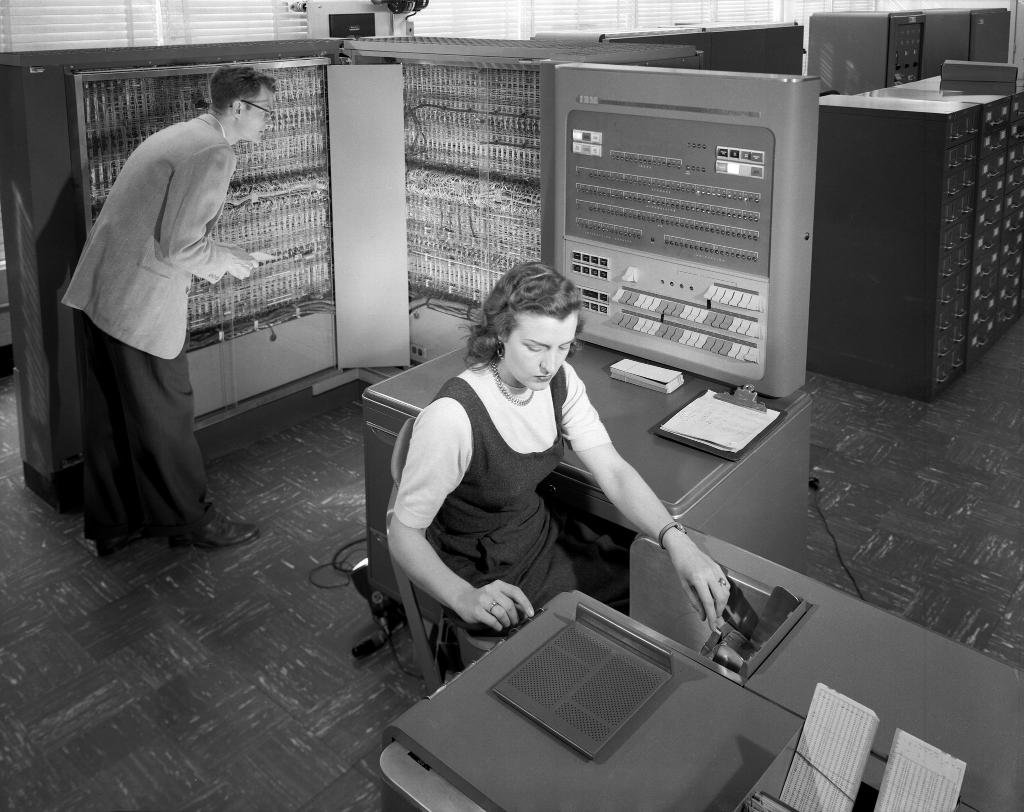
\includegraphics[width = .8\textwidth]{figures/punch_cards_nasa}};
\node[anchor = north west, font = \footnotesize] at (fig1.south west) {Source: \href{https://twitter.com/NASAhistory/status/1240971354003955712/photo/1}{NASA}};
\end{tikzpicture}
\end{frame}

\begin{frame}{How computing looked \textbf{in the 1980s}}
\begin{tikzpicture}[x = \textwidth, y = .8\textheight]
\node[anchor = north] (fig2) at (0,0) {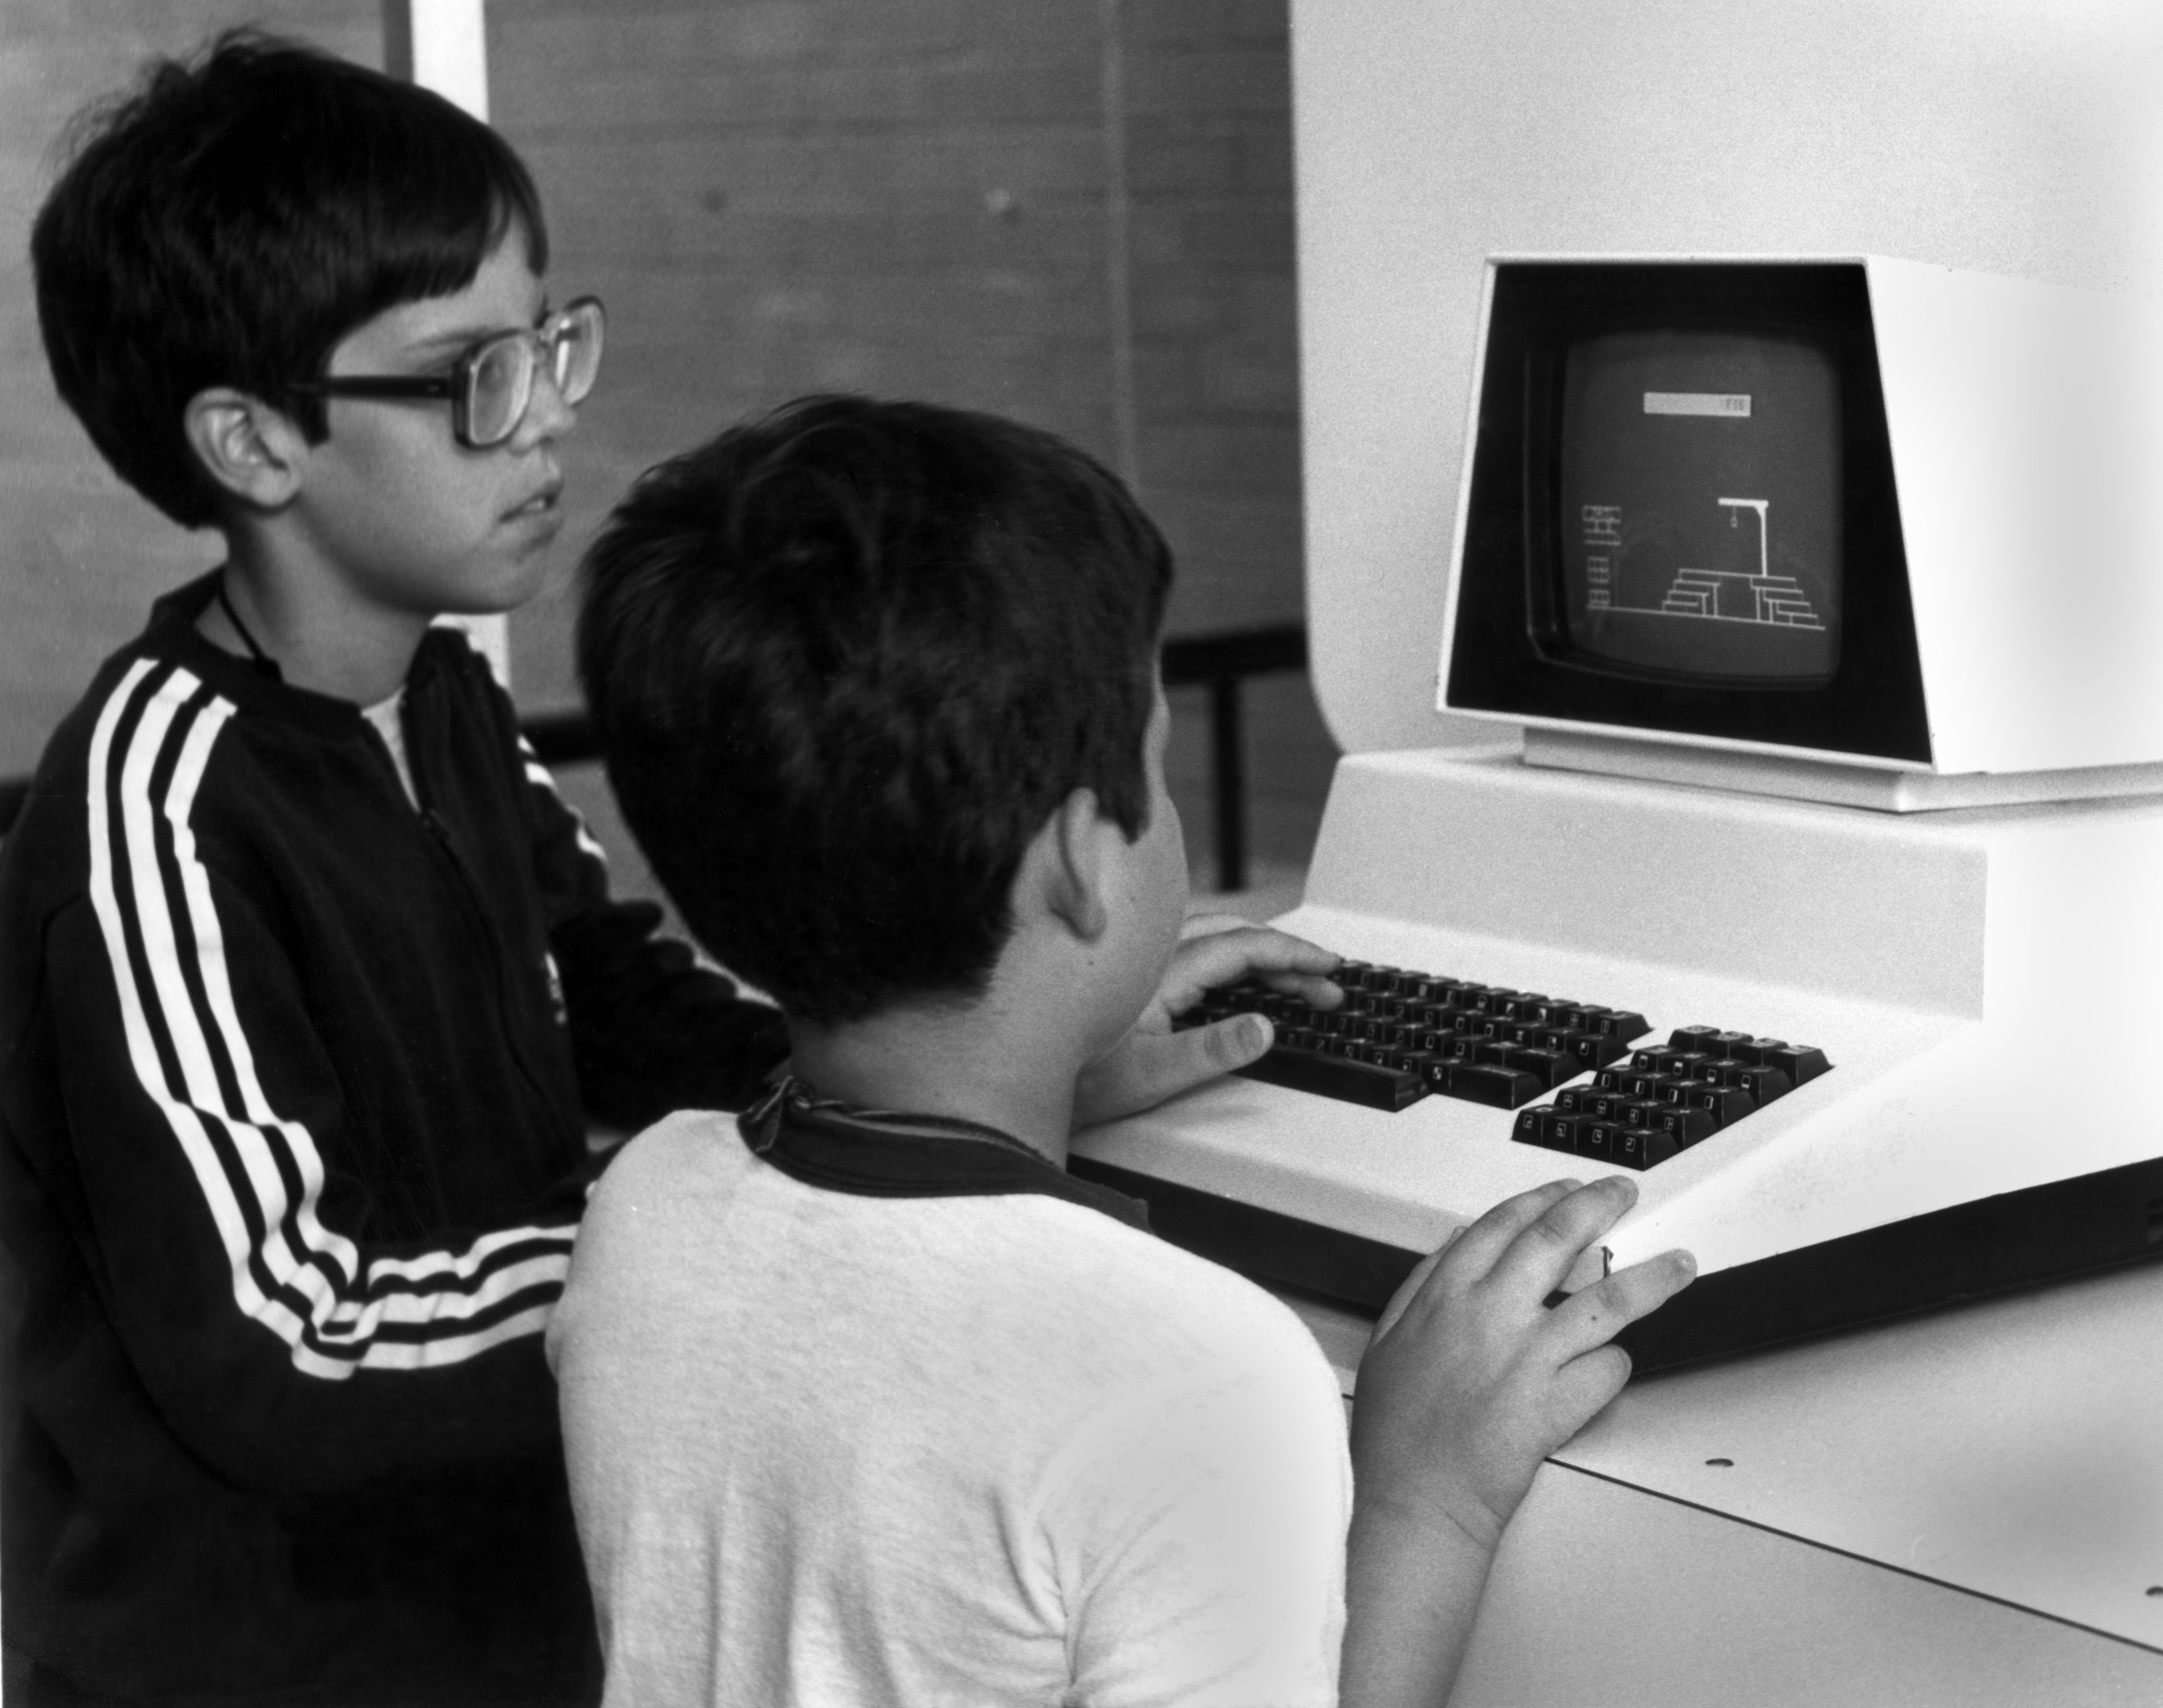
\includegraphics[width = .8\textwidth]{figures/pc}};
\node[anchor = north west, font = \footnotesize] at (fig2.south west) {Source: \href{https://commons.wikimedia.org/wiki/File:Commodore_PET_Exhibit_at_American_Museum_of_Science_and_Energy_Oak_Ridge_Tennessee.jpg}{Wikimedia}};
\end{tikzpicture}
\end{frame}

\begin{frame}{How computing looks \textbf{today}}
\begin{tikzpicture}[x = \textwidth, y = .8\textheight]
\node[anchor = north] (fig2) at (0,0) {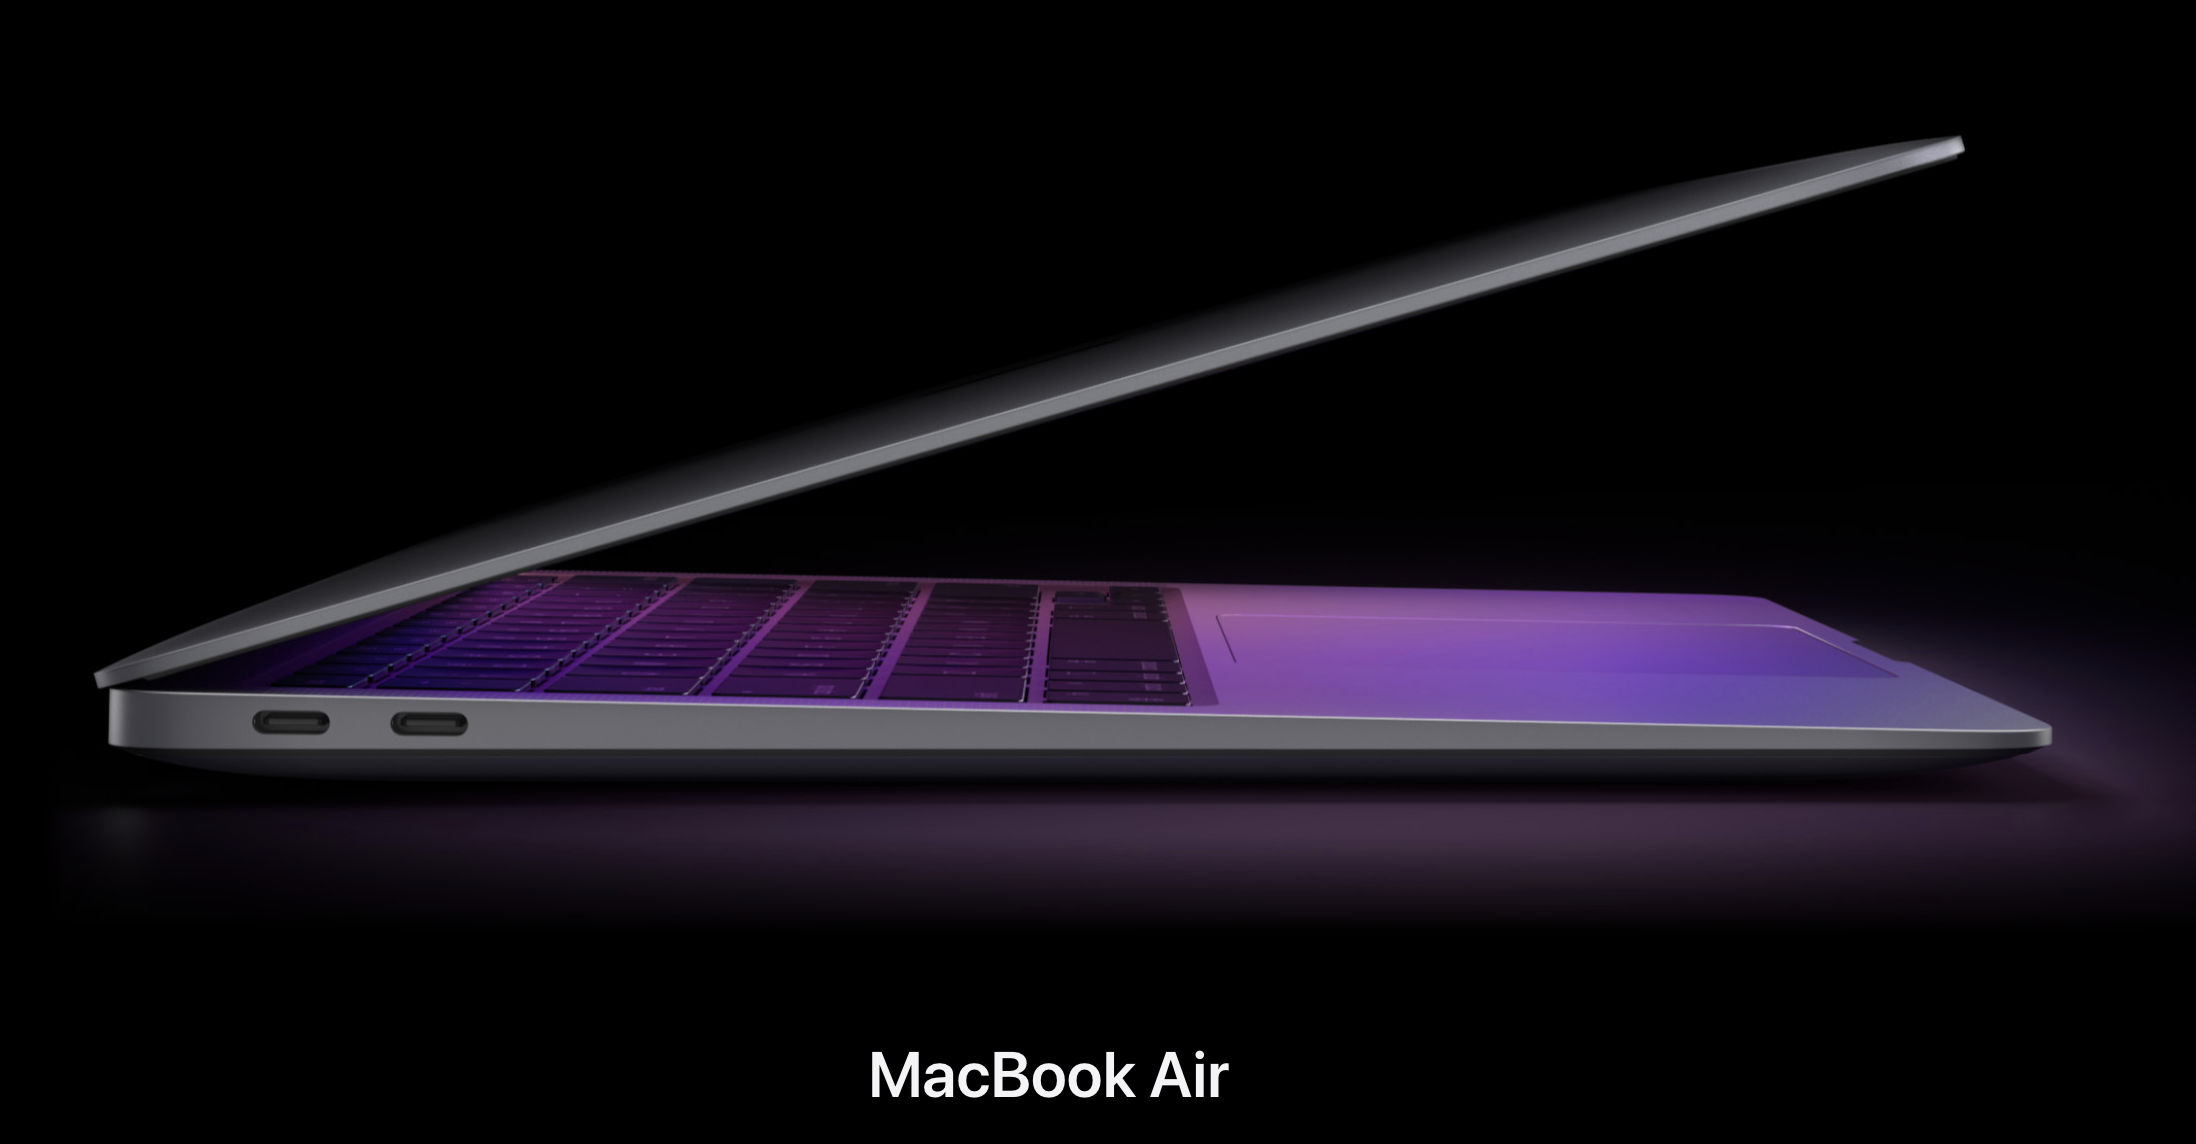
\includegraphics[width = \textwidth]{figures/macbook}};
\node[anchor = north west, font = \footnotesize] at (fig2.south west) {Source: \href{https://www.apple.com/macbook-air-m1/}{Apple}};
\end{tikzpicture}
\end{frame}

\begin{frame}{How computing looks \textbf{today}}
\begin{tikzpicture}[x = \textwidth, y = .8\textheight]
\node[anchor = north] (fig2a) at (.5,1) {
\includegraphics[width = .7\textwidth]{figures/gpt_request}};
\node<2->[anchor = north] (fig2b) at (fig2a.south) {
\includegraphics[width = .7\textwidth]{figures/gpt_poem}};
\node at (0,0) {};
\node at (1,1) {};
%\node[anchor = north west, font = \footnotesize] at (fig2b.south west) {Source: \href{https://chat.openai.com/chat}{OpenAI}};
\end{tikzpicture}
\end{frame}

\begin{frame}{The SOCIOL 212 sequence}
\begin{itemize}
\item new computational tools
\item applied to write a social science paper
\end{itemize}
\end{frame}

\begin{frame}{Course Plan}
\Huge
\bref{https://ilundberg.github.io/soc212b}{ilundberg.github.io/soc212b}
\end{frame}

\goalsframe

\section{Define an Estimand}

\begin{frame}{Asking research questions}

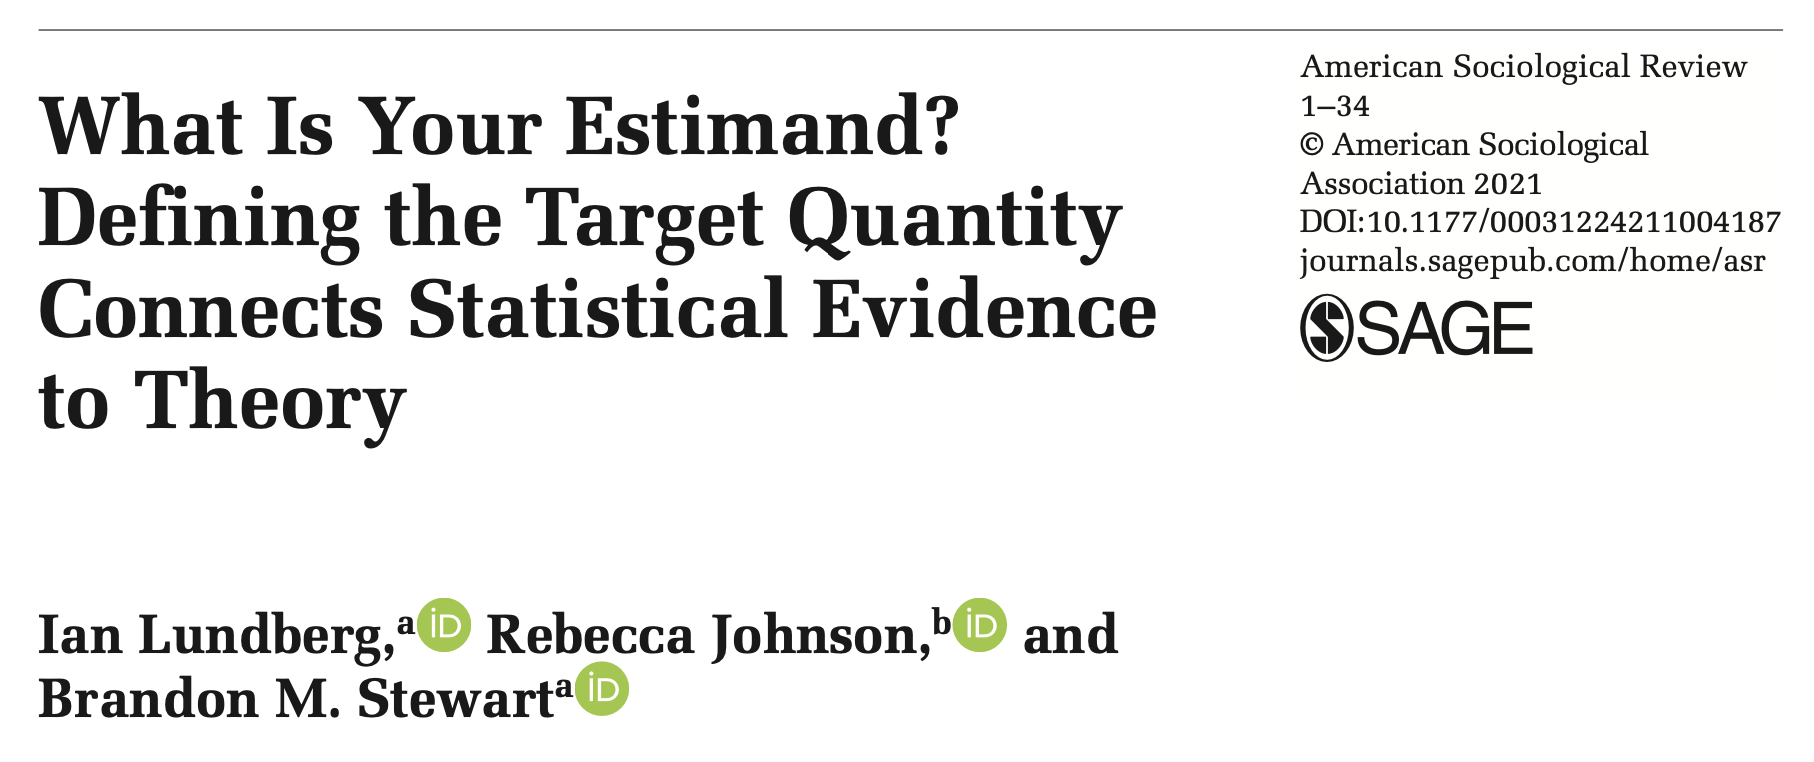
\includegraphics[width = \textwidth]{figures/estimand_title}

\end{frame}

\begin{frame}{Research framework: Estimands connect theory to evidence}
{\begin{tikzpicture}[x = 1.1in, y = .3in]
    \node[cloud, draw, align=center, cloud puffs=20,cloud puff arc=110, aspect=2, inner sep=.5mm] (general) at (-.2,0) {Theory or\\general goal};
    \node[align=center, white] (theoretical) at (1,0) {Theoretical\\estimand};
    \node[align=center, white] (empirical) at (2,0) {Empirical\\estimand};
    \node[align=center] (estimate) at (3,0) {Estimation\\strategy};
    \draw[->, thick] (general) -- (theoretical);
    \draw[->, thick] (theoretical) -- (empirical);
    \draw[->, thick] (empirical) -- (estimate);
    %%%%%%%%%%
 \node<2-4>[anchor = north, align = center, font = {\bf\footnotesize}, seagreen] at (-.2,-2) {Pages of theory};
 \draw<2-4>[->, seagreen, line width = 1.5pt] (-.2,-2) -- (.-.2,-1.2);
 \node<3-4>[anchor = north, align = center, font = {\bf\footnotesize}, seagreen] at (3,-2) {Pages of things\\done to data};
 \draw<3-4>[->, seagreen, line width = 1.5pt] (3,-2) -- (3,-1.2);
 \node<4>[anchor = north, align = center, font = {\bf\footnotesize}, red] at (1.5,-2) {Nothing in between};
 \draw<4>[->, red, line width = 1.5pt] (1.3,-2) -- (1.1,-1.2);
 \draw<4>[->, red, line width = 1.5pt] (1.7,-2) -- (1.9,-1.2);
    %%%%%%%%%%
    \node<5->[align=center] (theoretical) at (1,0) {Theoretical\\estimand};
    \node<6->[align=center, font = \footnotesize, anchor = north] (define) at (.5,-1) {\textbf{Set}\\a specific\\target};
    %\node[align=center, font = \scriptsize, anchor = north west] at (-.6,-5.4) {\textbf{Example tools:}};
    %\node[align=center, font = \scriptsize, anchor = north] at (.5,-5.4) {Target population,\\Causal contrast};
    \draw<6->[->, thick] (define) -- (.5,-.3);
    %\draw[thick] (.5,-5.3) -- (.5,-4.5);
    \draw<7-17>[line width = 2pt, gray] (-.5,-3.5) -- node[midway, above, text = black] {Definition} (.5,-3.5);
     \node<7-11>[align = center, rounded corners, font = \footnotesize, anchor = north, text width = 1.1in] at (0, -3.7) {A \bblue{unit-specific quantity}\\aggregated over a\\\bblue{target population}};
    \draw<8-17>[line width = 2pt, gray] (.6,-3.5) -- node[midway, above, text = black] {Example} (3.5,-3.5);
     \node<8>[anchor = north west, font = \footnotesize] at (.6,-4) {$\begin{aligned}\frac{1}{\substack{\text{Size of U.S.}\\\text{adult population}}}\sum_{\substack{i\text{ in U.S.}\\\text{adult population}}}\bigg(\text{Employed}_i\bigg)\end{aligned}$};
     \node<9-10>[anchor = north west, font = \footnotesize] at (.6,-4) {$\begin{aligned}\frac{1}{\substack{\text{Size of U.S.}\\\text{adult population}}}\sum_{\substack{i\text{ in U.S.}\\\text{adult population}}} \bigg(&\underbrace{\text{Employed}_i(\text{Job training})}_{\substack{\text{Employment if received}\\\text{job training}}} \\ &- \underbrace{\text{Employed}_i(\text{No job training})}_{\substack{\text{Employment if did not receive}\\\text{job training}}}\bigg) \end{aligned}$};
    \node<10-11>[align=right, gray, font = \footnotesize, anchor = south east] (define) at (3.5,-9.5) {Lieberson 1987, Abbott 1988, Freedman 1991, Xie 2013, Hern\'an 2018};
     %\node<11>[anchor = north] at (2.05,-3.7) {\estimandFigureNoCaptionCustom{$Y_i(1)$\\$-Y_i(0)$}{\tiny}{6pt}{1}{.7}};
     \node<11-12>[anchor = north west] at (.8,-3.7) {\estimandFigureNoCaptionCustom{$Y_i(1)$}{\tiny}{6pt}{.5}{.7}};
     \draw<11-17>[line width = 1.2pt] (1.95,-5.3) -- (2.15,-5.3);
     \node<11-13>[anchor = north east] at (3.3,-3.7) {\estimandFigureNoCaptionCustom{$Y_i(0)$}{\tiny}{6pt}{.5}{.7}};
    %%%%%%%%%%
    \node<5->[align=center] (empirical) at (2,0) {Empirical\\estimand};
    \node<12->[align=center, font = \footnotesize, anchor = north] (identify) at (1.5,-1) {\textbf{Link}\\to observable\\data};
    %\node[align=center, font = \footnotesize, anchor = north] at (1.5,-5.4) {Directed Acyclic Graphs,\\Potential outcomes};
    \draw<12->[->, thick] (identify) -- (1.5,-.3);
     \node<12-15>[align = center, rounded corners, font = \footnotesize, anchor = north, text width = 1.1in] at (0, -3.7) {A quantity involving \bblue{observable data}};
     \node<13-16>[anchor = north west] at (.8,-3.7) {\estimandFigureNoCaptionMissingA{$Y_i(1)$}{\tiny}{6pt}{.5}{.7}};
     \node<14-16>[anchor = north east] at (3.3,-3.7) {\estimandFigureNoCaptionMissingB{$Y_i(0)$}{\tiny}{6pt}{.5}{.7}};
      \node<15> (x) at (1.5,-7.3) {$\vec{X}$};
      \node<15> (d) at (2,-7.3) {$T$};
      \node<15> (y) at (2.5,-7.3) {$Y$};
      \draw<15>[->, thick] (x) -- (d);
      \draw<15>[->, thick] (x) to[bend right] (y);
      \draw<15>[->, thick] (d) -- (y);
    \node<15>[align=right, gray, font = \footnotesize, anchor = south east] (define) at (3.5,-9.5) {Pearl 2009, Imbens and Rubin 2015,\\Morgan and Winship 2015, Elwert and Winship 2014};
    %%%%%%%%%%
    \node<16->[align=center, font = \footnotesize, anchor = north] (learn) at (2.5,-1) {\textbf{Learn}\\from data};
    %\node[align=center, font = \footnotesize, anchor = north] at (2.5,-5.4) {OLS regression,\\Machine learning};
    \draw<16->[->, thick] (learn) -- (2.5,-.3);
    %\draw[thick] (2.5,-5.3) -- (2.5,-4.5);
     \node<16-17>[align = center, rounded corners, font = \footnotesize, anchor = north, text width = 1.1in] at (0, -3.7) {An algorithm applied to data};
     \node<17>[anchor = north west] at (.8,-3.7) {\estimandFigureNoCaptionImputedA{$Y_i(1)$}{\tiny}{6pt}{.5}{.7}};
     \node<17>[anchor = north east] at (3.3,-3.7) {\estimandFigureNoCaptionImputedB{$Y_i(0)$}{\tiny}{6pt}{.5}{.7}};
    %\node<17-18>[anchor = north west, font = \scriptsize] at (.6,-3.7) {$\begin{aligned}\hat\theta &= \underbrace{\frac{1}{n}\sum_{i=1}^n}_{\substack{\text{Sample}\\\text{average}}} \bigg(\underbrace{\hat\E(Y\mid \vec{X} = \vec{x}_i, D = 1)}_{\substack{\text{Regression prediction}\\\text{if treated}}} - \underbrace{\hat\E(Y\mid \vec{X} = \vec{x}_i, D = 0)}_{\substack{\text{Regression prediction}\\\text{if untreated}}}\bigg)\end{aligned}$};
    \node<17>[align=right, gray, font = \footnotesize, anchor = south east] (define) at (3.5,-9.5) {Young 2009, Watts 2014, Berk et al. 2019, Molina and Garip 2019};
    % Types of argument
    \onslide<19->{
    \node[align=center, font = \footnotesize, anchor = north] at (.5,-3.7) {By argument};
    \draw[thick] (.5,-3.8) -- (.5,-2.8);
    \node[align=center, font = \footnotesize, anchor = north] at (1.5,-3.7) {By assumption};
    \draw[thick] (1.5,-3.8) -- (1.5,-2.8);
    \node[align=center, font = \footnotesize, anchor = north] at (2.5,-3.7) {By data};
    \draw[thick] (2.5,-3.8) -- (2.5,-2.8);
    }
    \end{tikzpicture}
    }
\end{frame}

\begin{frame}{Defining an estimand}

An estimand involves a
\begin{itemize}
\item unit-specific quantity
\item target population
\end{itemize} \vskip .2in
We will practice with
\begin{itemize}
\item simple guiding examples
\item then with your projects
\end{itemize}

\end{frame}

% DESCRIBE POPULATION
\begin{frame}[t]\headerfigureset
\begin{tikzpicture}[x = \textwidth, y = .8\textheight]
\node at (0,0) {};
\node at (1,1) {};
\node[anchor = west, font = {\large\bf}] (goal) at (0, .9) {Describe a population};
\draw[line width = 1.5pt, line cap = round] (goal.south west) -- (goal.south east);
\node[anchor = west] at (0, .75) {What is the proportion employed};
\node[anchor = west] at (0, .68) {among U.S. resident women ages 21--35?};
% Title rows
\only<2->{
\node[font = \footnotesize, anchor = east] at (.4, .4) {Woman 1};
\node[font = \footnotesize, anchor = east] at (.4, .35) {Woman 2};
\node[font = \footnotesize, anchor = east] at (.4, .3) {Woman 3};
\node[font = \footnotesize, anchor = east] at (.4, .25) {Woman 4};
}
\only<3->{
% Title columns
\node[font = \footnotesize, anchor = south] (emp) at (.5, .45) {Employed?};
\draw[thick] (.4,.45) -- (.6, .45);
% Cell values
\node[font = \footnotesize] at (.5, .4) {1};
\node[font = \footnotesize] at (.5, .35) {0};
\node[font = \footnotesize] at (.5, .3) {1};
\node[font = \footnotesize] at (.5, .25) {1};
}
\end{tikzpicture}
\end{frame}

% DESCRIBE POPULATION SUBGROUPS
\begin{frame}[t]\headerfigureset
\begin{tikzpicture}[x = \textwidth, y = .8\textheight]
\node at (0,0) {};
\node at (1,1) {};
\node[anchor = west, font = {\large\bf}] (goal) at (0, .9) {Describe population subgroups};
\draw[line width = 1.5pt, line cap = round] (goal.south west) -- (goal.south east);
\node[anchor = west] at (0, .75) {What is the proportion employed};
\node[anchor = west] at (0, .68) {among U.S. resident women ages 21--35,};
\node[anchor = west] at (0, .61) {comparing mothers to non-mothers?};
% MOTHERS
% Title rows
\only<2->{
\node[font = \footnotesize, anchor = east] at (.2, .4) {Mother 1};
\node[font = \footnotesize, anchor = east] at (.2, .35) {Mother 2};
\node[font = \footnotesize, anchor = east] at (.2, .3) {Mother 3};
\node[font = \footnotesize, anchor = east] at (.2, .25) {Mother 4};
% Title columns
\node[font = \footnotesize, anchor = south] (emp) at (.3, .45) {Employed?};
\draw[thick] (.2,.45) -- (.4, .45);
% Cell values
\node[font = \footnotesize] at (.3, .4) {0};
\node[font = \footnotesize] at (.3, .35) {0};
\node[font = \footnotesize] at (.3, .3) {0};
\node[font = \footnotesize] at (.3, .25) {1};
% NON-MOTHERS
% Title rows
\node[font = \footnotesize, anchor = east] at (.7, .4) {Non-Mother 1};
\node[font = \footnotesize, anchor = east] at (.7, .35) {Non-Mother 2};
\node[font = \footnotesize, anchor = east] at (.7, .3) {Non-Mother 3};
\node[font = \footnotesize, anchor = east] at (.7, .25) {Non-Mother 4};
% Title columns
\node[font = \footnotesize, anchor = south] (emp) at (.8, .45) {Employed?};
\draw[thick] (.7,.45) -- (.9, .45);
% Cell values
\node[font = \footnotesize] at (.8, .4) {1};
\node[font = \footnotesize] at (.8, .35) {0};
\node[font = \footnotesize] at (.8, .3) {1};
\node[font = \footnotesize] at (.8, .25) {1};
}
\end{tikzpicture}
\end{frame}

% CAUSAL EFFECT IN A POPULATION
\begin{frame}[t]\headerfigureset
\begin{tikzpicture}[x = \textwidth, y = .8\textheight]
\node at (0,0) {};
\node at (1,1) {};
\node[anchor = west, font = {\large\bf}] (goal) at (0, .9) {Causal effect in a population};
\draw[line width = 1.5pt, line cap = round] (goal.south west) -- (goal.south east);
\node[anchor = west] at (0, .75) {What is the causal effect of motherhood on employment};
\node[anchor = west] at (0, .68) {among U.S. resident women ages 21--35?};
\only<2->{
% Title rows
\node[font = \footnotesize, anchor = east] at (.2, .3) {Woman 1};
\node[font = \footnotesize, anchor = east] at (.2, .25) {Woman 2};
\node[font = \footnotesize, anchor = east] at (.2, .2) {Woman 3};
\node[font = \footnotesize, anchor = east] at (.2, .15) {Woman 4};
}
\only<3->{
% Title column 1
\node[font = \footnotesize, anchor = south, align = center] (emp) at (.3, .35) {Would be\\employed if\\a mother?\\$Y(1)$};
\draw[thick] (.22,.35) -- (.38, .35);
% Cell values 1
\node[font = \footnotesize] at (.3, .3) {0};
\node[font = \footnotesize] at (.3, .25) {0};
\node[font = \footnotesize] at (.3, .2) {0};
\node[font = \footnotesize] at (.3, .15) {1};
}
\only<4->{
% Title column 0
\node[font = \footnotesize, anchor = south, align = center] (emp) at (.5, .35) {Would be\\employed if\\a non-mother?\\$Y(0)$};
\draw[thick] (.42,.35) -- (.58, .35);
% Cell values 0
\node[font = \footnotesize] at (.5, .3) {1};
\node[font = \footnotesize] at (.5, .25) {0};
\node[font = \footnotesize] at (.5, .2) {1};
\node[font = \footnotesize] at (.5, .15) {1};
}
\only<5->{
% Title column causal
\node[font = \footnotesize, anchor = south, align = center] (emp) at (.7, .35) {Causal\\effect\\$Y(1) - Y(0)$};
\draw[thick] (.62,.35) -- (.78, .35);
% Cell values causal
\node[font = \footnotesize] at (.7, .3) {-1};
\node[font = \footnotesize] at (.7, .25) {0};
\node[font = \footnotesize] at (.7, .2) {-1};
\node[font = \footnotesize] at (.7, .15) {0};
}
\end{tikzpicture}
\end{frame}

\begin{frame}{Defining an estimand: Your project}

Form small groups. In your projects,
\begin{itemize}
\item What is the unit-specific quantity (or quantities)?
\item What is the target population(s)?
\end{itemize}

\end{frame}

\section{$\hat{Y}$ View of Regression}

\tcframe

\begin{frame}{Baseball salaries}
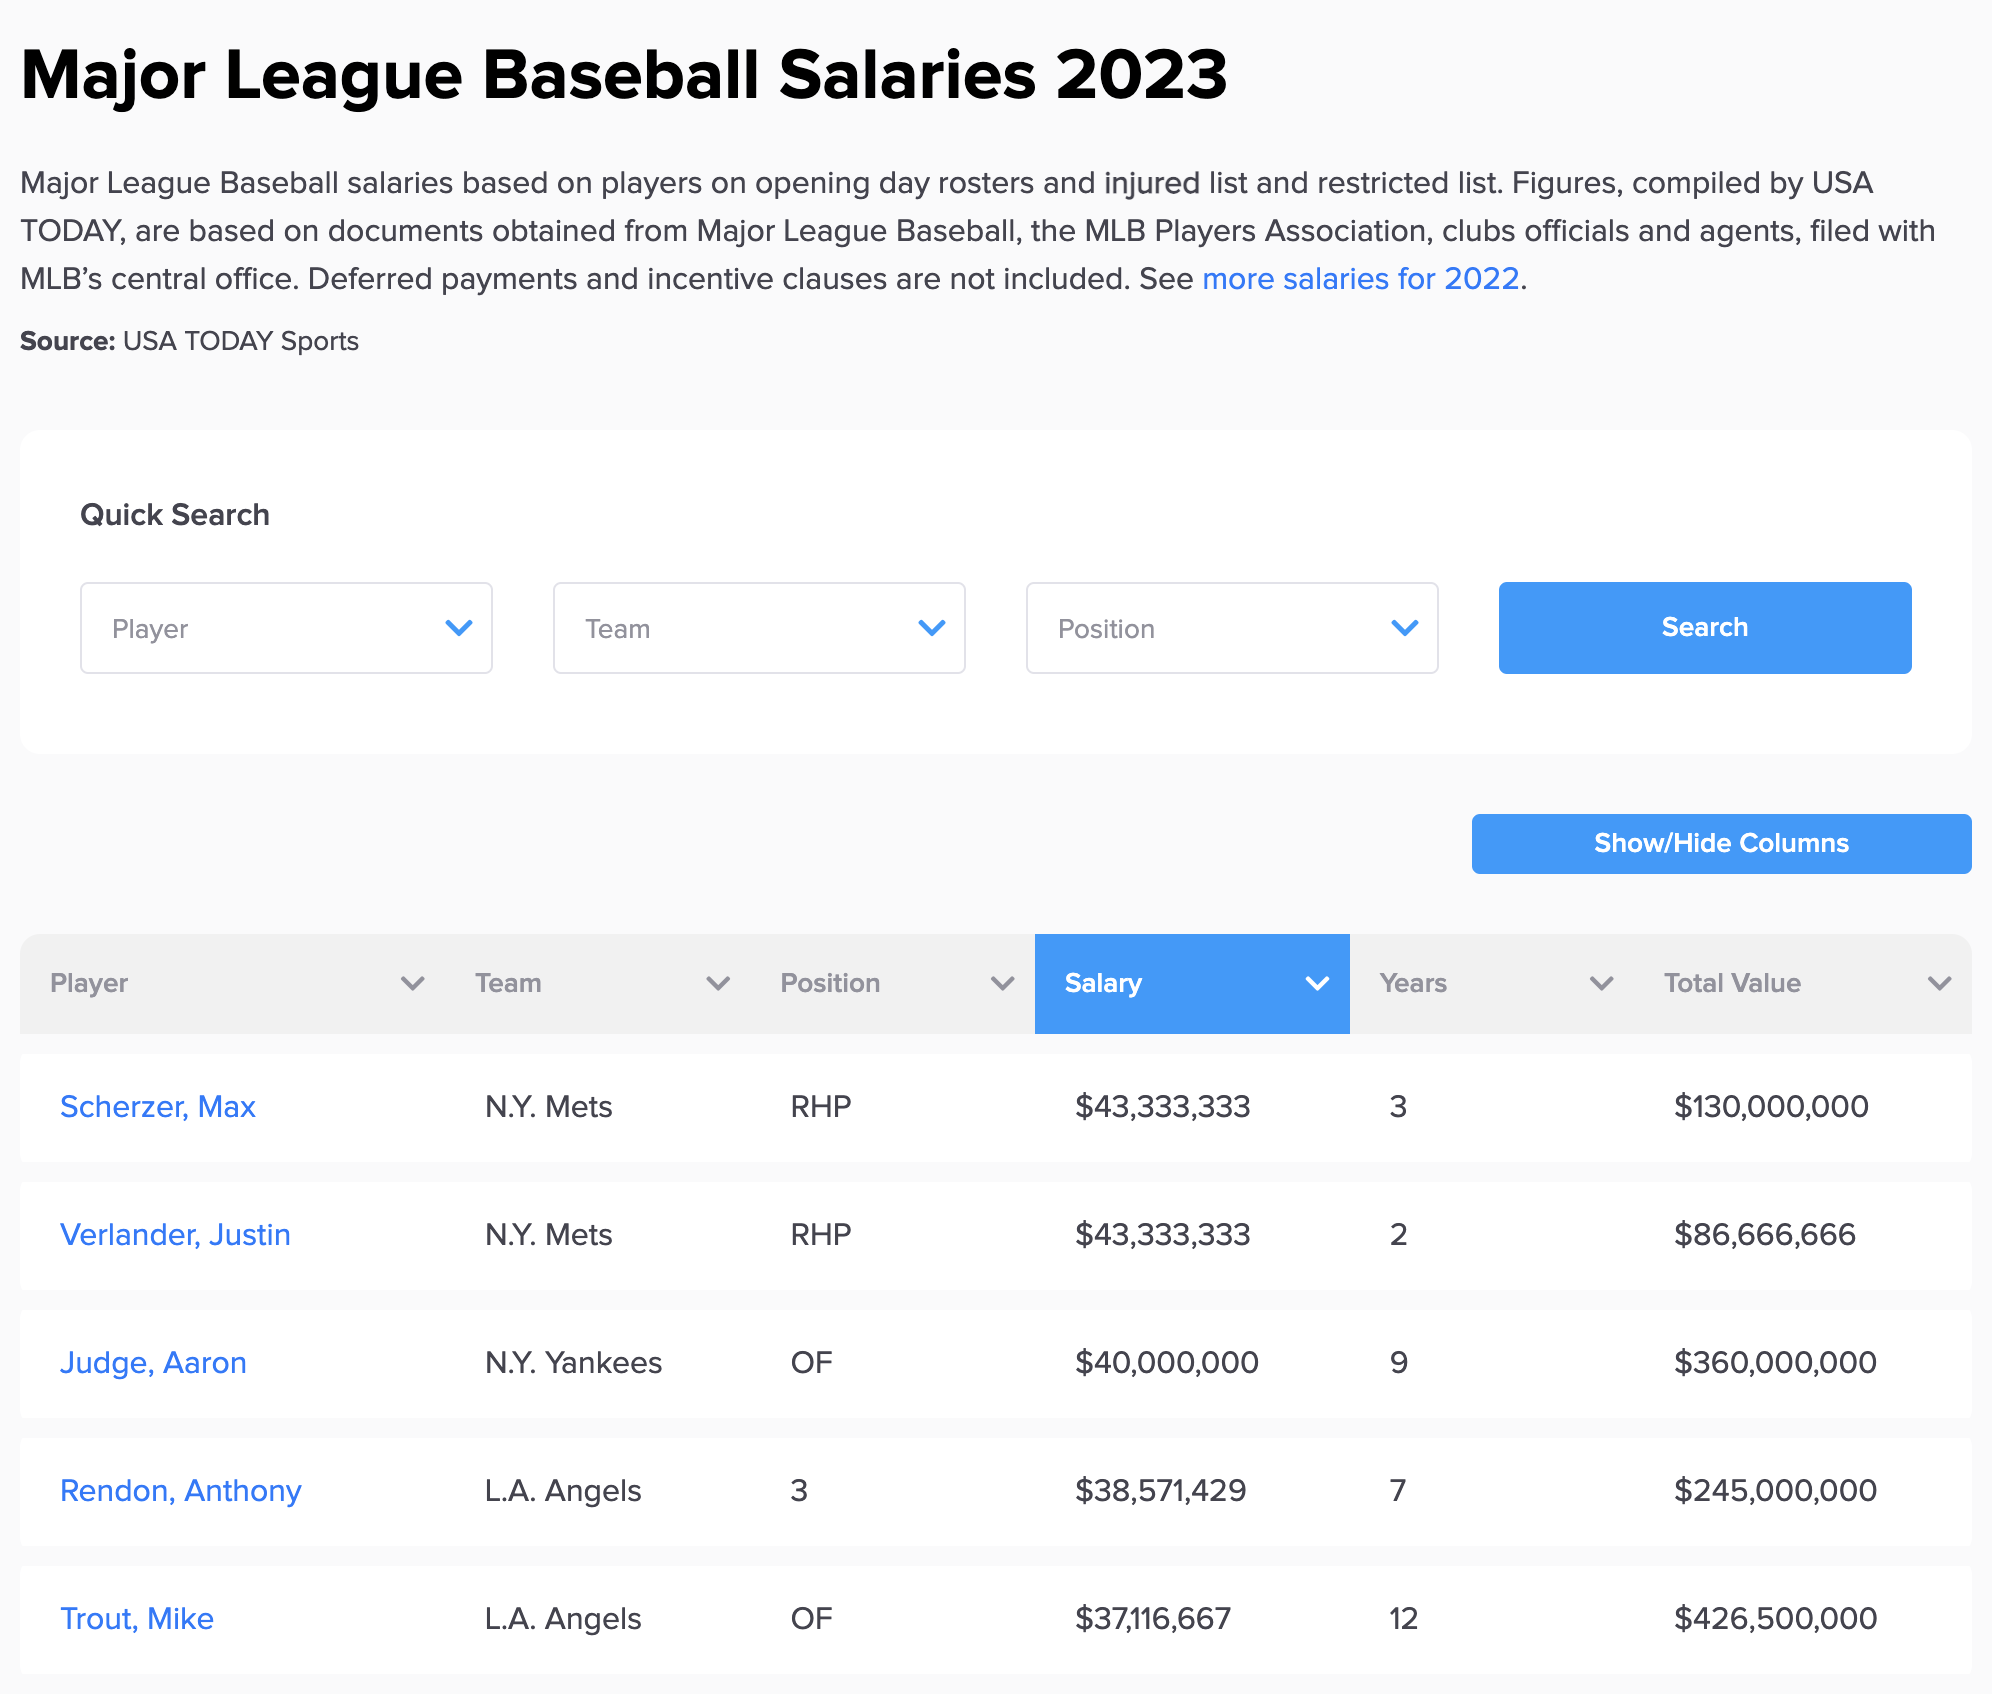
\includegraphics[width = .6\textwidth]{figures/baseball_source}\\
\bref{https://databases.usatoday.com/major-league-baseball-salaries-2023/}{databases.usatoday.com/major-league-baseball-salaries-2023/}
\end{frame}


\begin{frame}{Baseball salaries}
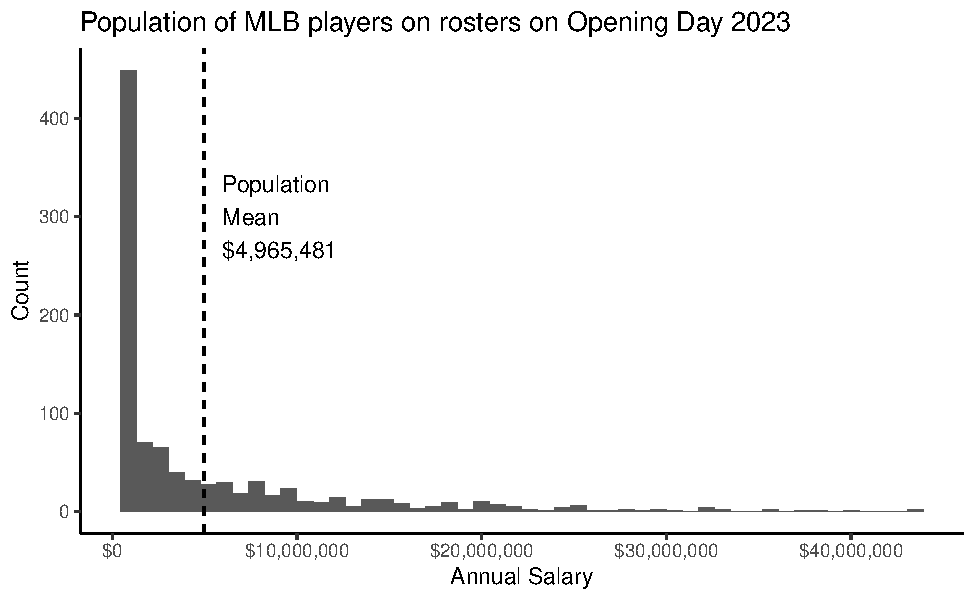
\includegraphics[width = \textwidth]{figures/baseball_histogram}
\end{frame}

\begin{frame}{Baseball salaries}

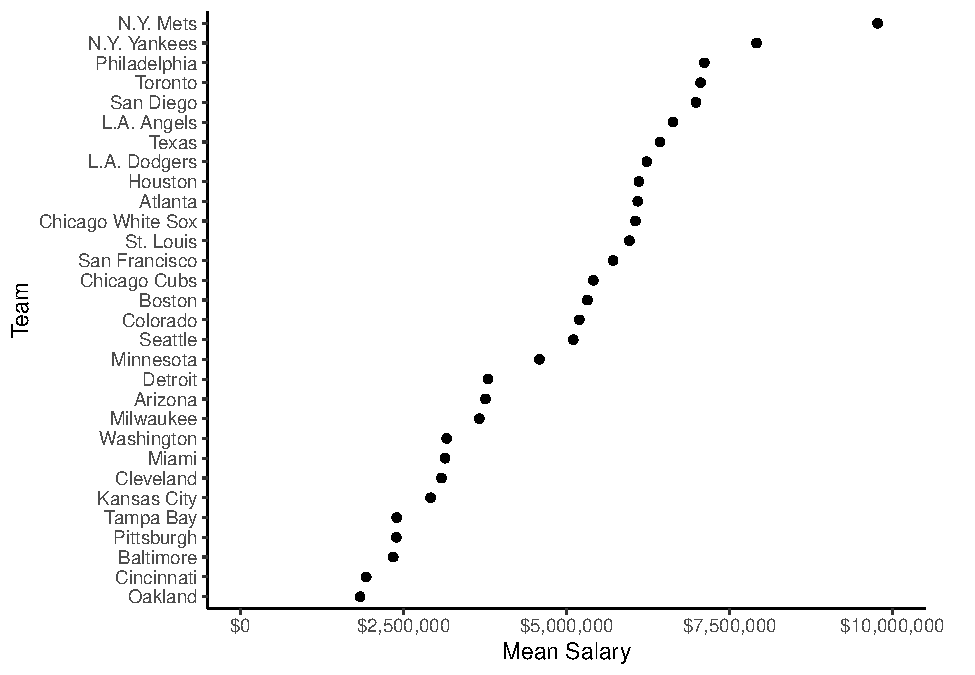
\includegraphics[width = \textwidth]{figures/all_team_mean}

\end{frame}

\begin{frame}{Statistical learning from samples}

With only the sample, how would you estimate the mean salary of all the Dodgers? \vskip .2in

\begin{tabular}{ll}
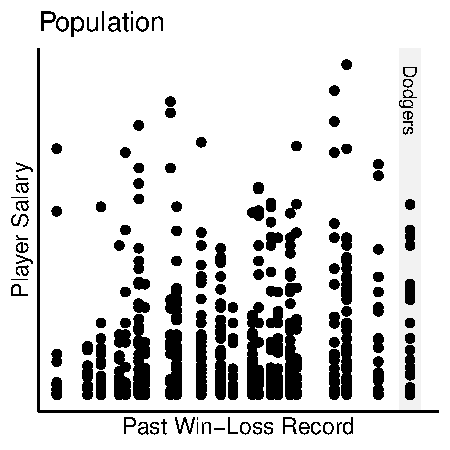
\includegraphics[width = .48\textwidth]{figures/dodgers_population} &
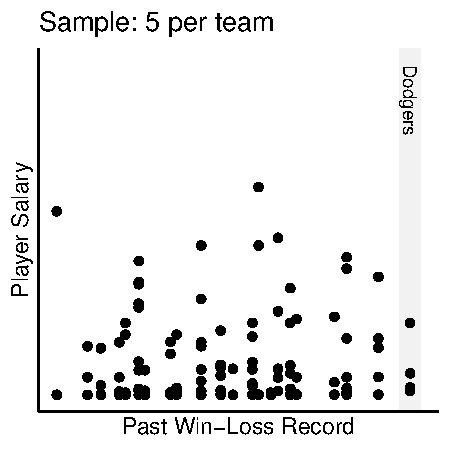
\includegraphics[width = .48\textwidth]{figures/dodgers_sample}
\end{tabular}

\end{frame}

\begin{frame}{Three estimators for the Dodgers' mean salary}

\includegraphics<1>[width = \textwidth]{figures/dodgers_estimator1}
\includegraphics<2>[width = \textwidth]{figures/dodgers_estimator2}
\includegraphics<3>[width = \textwidth]{figures/dodgers_estimator3}
\only<4->{
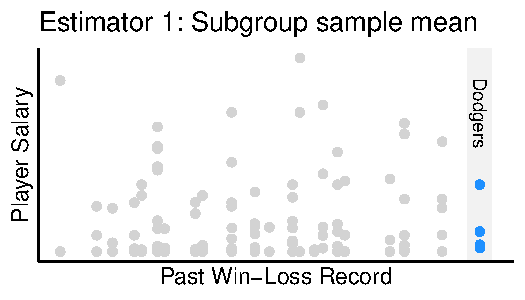
\includegraphics[width = .32\textwidth]{figures/dodgers_estimator1}
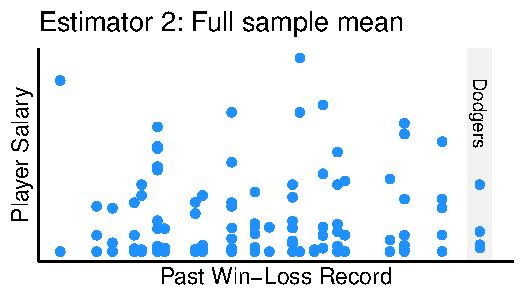
\includegraphics[width = .32\textwidth]{figures/dodgers_estimator2}
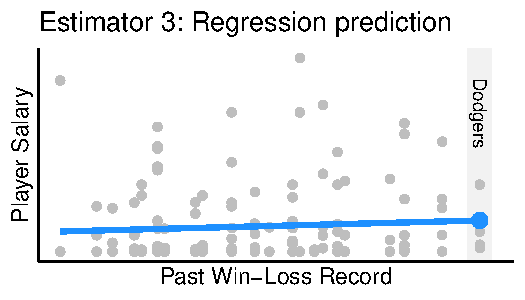
\includegraphics[width = .32\textwidth]{figures/dodgers_estimator3} \vskip .2in
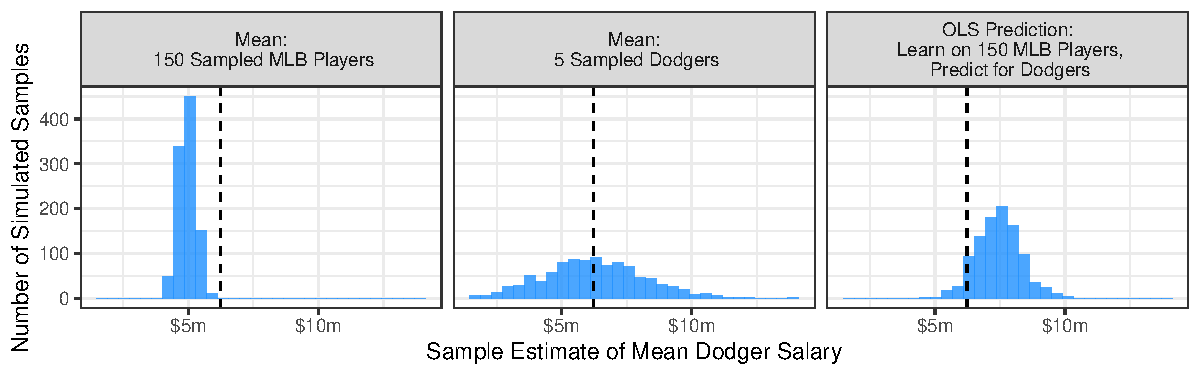
\includegraphics[width = \textwidth]{figures/dodgers_estimator_histogram}
} \vskip .1in
\onslide<5->{
Which do you prefer? Why?
}
\end{frame}

\begin{frame}{Statistical learning: A somewhat unusual view} \pause

\begin{enumerate}
\item the entire goal of modeling is to solve sparse data
\begin{itemize}
\item we sample very few Dodgers,\\so we use non-Dodgers to help our estimate
\end{itemize} \pause \vskip .1in
\item in a huge sample, a model is unnecessary
\begin{itemize}
\item estimate Dodger population mean\\by the Dodger sample mean
\end{itemize} \pause \vskip .1in
\item in a tiny sample, models may perform poorly
\begin{itemize}
\item might even better to estimate a subgroup mean (Dodgers)\\by taking the mean of the whole sample (all MLB)
\end{itemize}
\end{enumerate}

\end{frame}

\begin{frame}

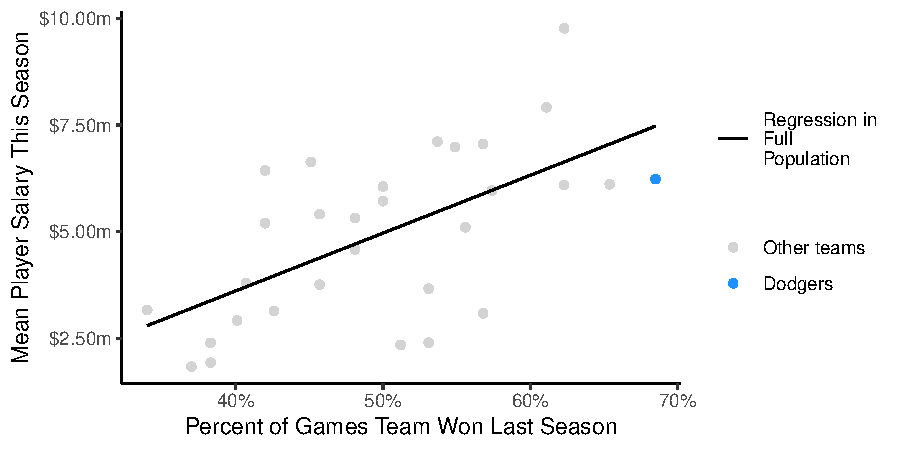
\includegraphics[width = \textwidth]{figures/dodger_model_wrong} \pause \vskip .1in

The model is wrong. Why might we still use it?

\end{frame}

\begin{frame}{$\hat{Y}$ view of regression: Modeling errors}{Berk Fig 1.6}
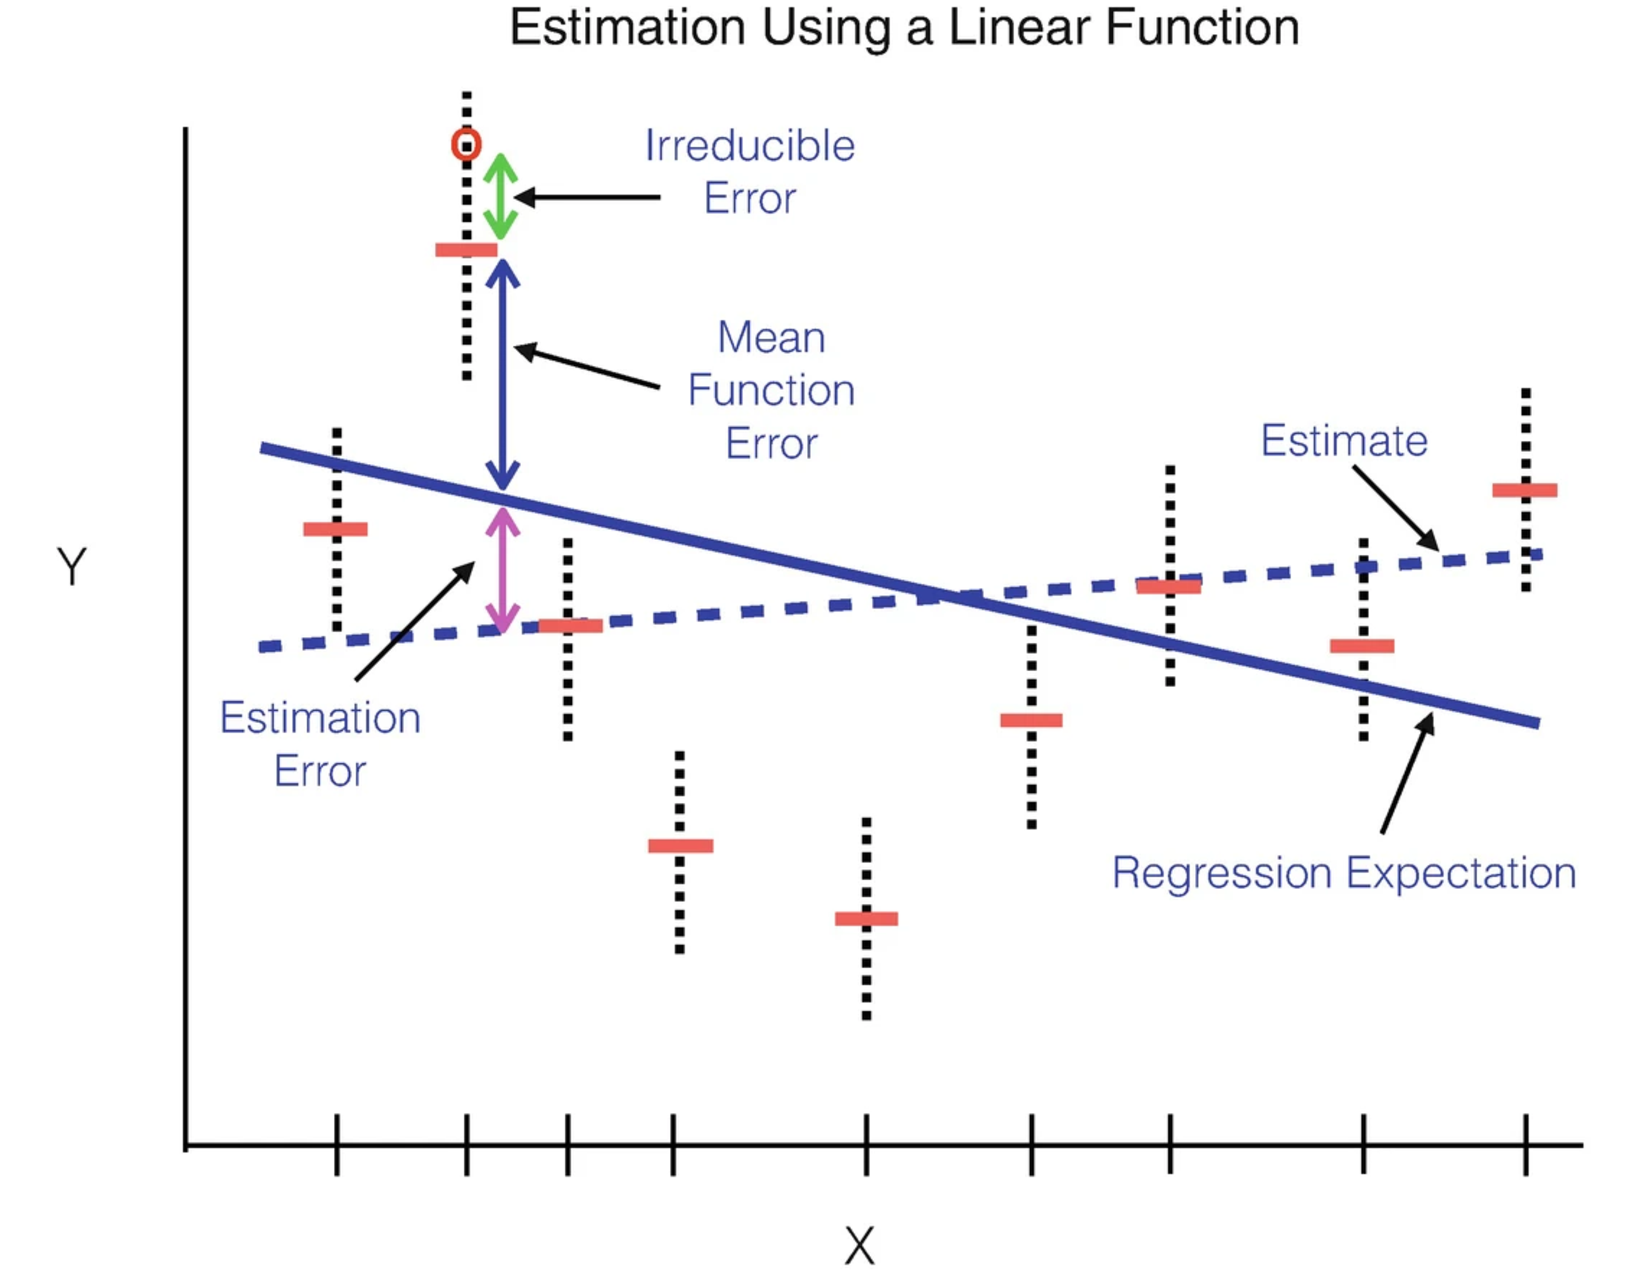
\includegraphics[width = .8\textwidth]{figures/berk_fig1.6}
\end{frame}

\section{Computer Tutorial}

\tcframe

\begin{frame}{A $\hat{Y}$ view of description: Predict a subgroup mean}{With Kristin Liao, UCLA}

\begin{tikzpicture}[x = \textwidth, y = .8\textheight]
\node at (0,0) {};
\node at (1,1) {};
\node<2>[anchor = west] at (0,.5) {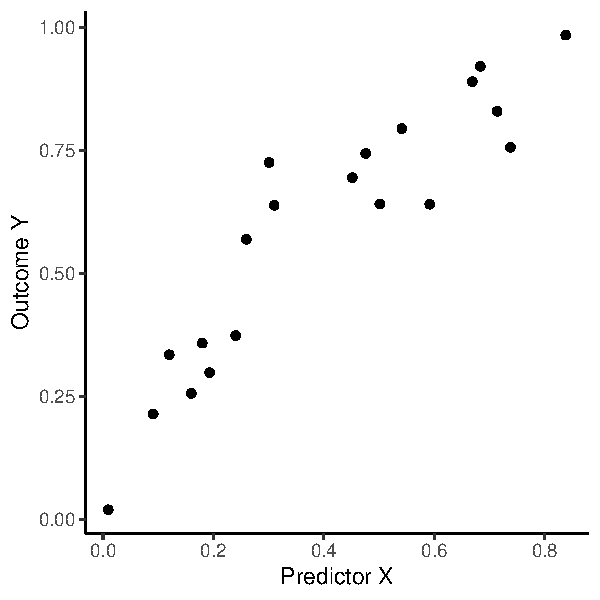
\includegraphics[height = .8\textheight]{figures/illustration_1}};
\node<3>[anchor = west] at (0,.5) {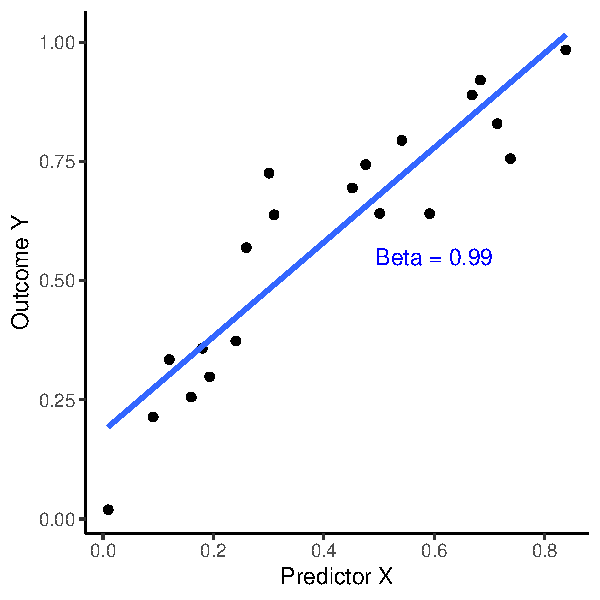
\includegraphics[height = .8\textheight]{figures/illustration_2}};
\node<4->[anchor = west] at (0,.5) {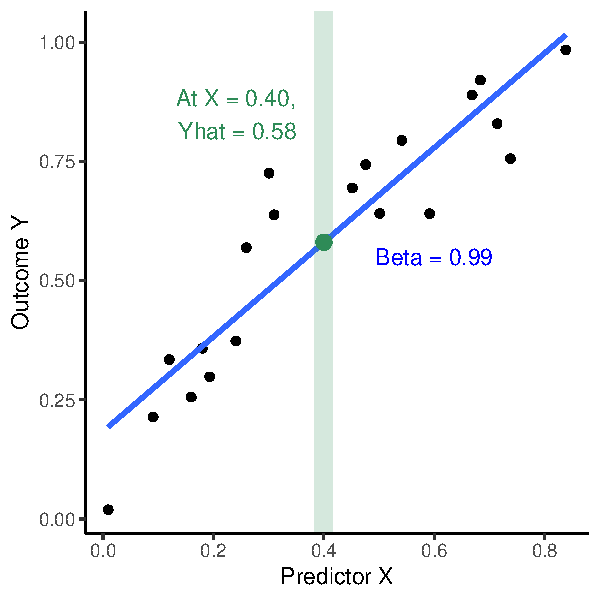
\includegraphics[height = .8\textheight]{figures/illustration_3}};
%\node<6-12>[anchor = north west, align = left, font = \bf] at (.7, 1) {Why model?};
%\node<7-12>[anchor = north west, align = left] at (.7, .9) {A subgroups may\\have few units};
%\node<8-12>[anchor = north west, align = left] at (.7, .725) {Model pools\\information\\across subgroups};
%\node<9-12>[anchor = north west, align = left] at (.7, .5) {Goal: $\hat{Y}$, not $\hat\beta$};
%\node<10-12>[anchor = north west, align = left, font = \bf] at (.7, .35) {Benefits};
%\node<11-12>[anchor = north west, align = left] at (.7, .25) {Jargon-free results};
%\node<12>[anchor = north west, align = left] at (.7, .15) {Plug in machine\\learning};
\node<5->[anchor = north west, align = left, font = \bf] at (.7, 1) {Concrete steps};
\node<6->[anchor = north west, align = left] at (.7, .9) {In full data,\\learn a model};
\node<7->[anchor = north west, align = left] at (.7, .725) {Define new data\\in which to predict};
\node<8->[anchor = north west, align = left] at (.7, .55) {Report prediction};
\end{tikzpicture}

\includegraphics<1>[height = .8\textheight]{figures/illustration_1}
\includegraphics<2>[height = .8\textheight]{figures/illustration_2}
\includegraphics<3>[height = .8\textheight]{figures/illustration_3}

\end{frame}

\begin{frame}{Concrete exercise: Sex gap in pay}{\href{https://ilundberg.github.io/description/}{\textcolor{blue}{ilundberg.github.io/description}}}
\begin{tabular}{ll}
Sample of 5 million cases & (true nonparametric estimates) \\
Simulate a sample of 100 & (evaluate sample-based estimators)
\end{tabular}
\end{frame}

\begin{frame}{Concrete exercise: Sex gap in pay}{\href{https://ilundberg.github.io/description/}{\textcolor{blue}{ilundberg.github.io/description}}}
Data for learning
\begin{itemize}
\item American Community Survey (ACS) 2010–2019
\item Adults age 30--50
\item Worked 35+ hours per week in 50+ weeks last year
\item Outcome: Annual wage and salary income
\end{itemize}
\end{frame}

\begin{frame}{Computer tutorial: Introduction}{\href{https://ilundberg.github.io/description/}{\textcolor{blue}{ilundberg.github.io/description}}} \pause

We will give you data:
\begin{itemize}
\item male and female incomes at age 30–50 in 2010–2019
\end{itemize} \vskip .1in
You will make a forecast:
\begin{itemize}
\item male and female geometric mean income at age 30–50 in 2022
\end{itemize}

\end{frame}

\begin{frame}{Computer tutorial: Introduction}{\href{https://ilundberg.github.io/description/}{\textcolor{blue}{ilundberg.github.io/description}}}

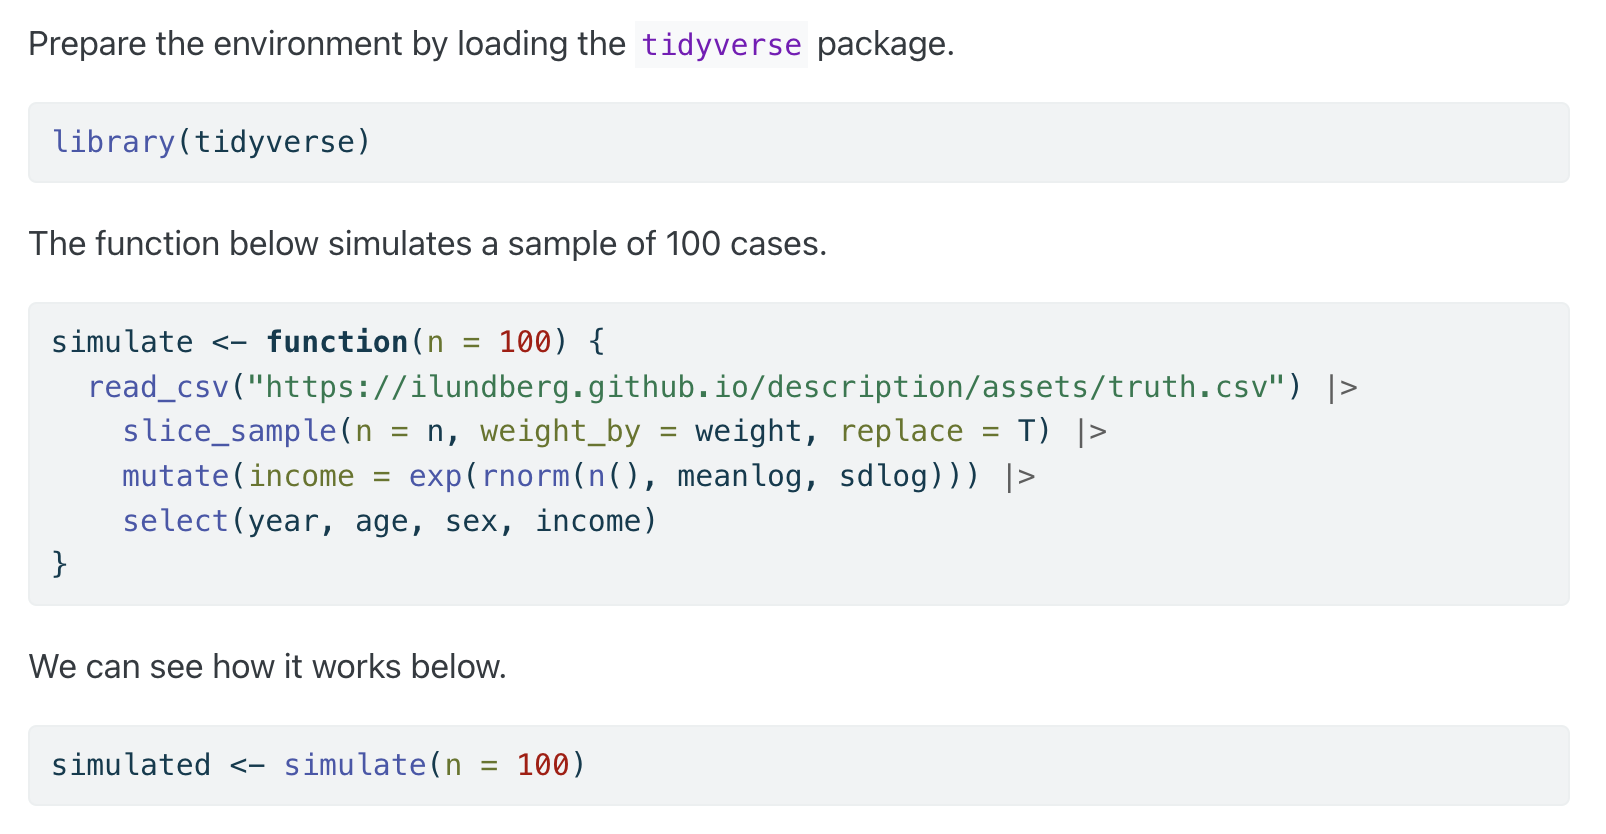
\includegraphics[width = \textwidth]{figures/code_simulate}

\end{frame}

\begin{frame}{Computer tutorial: Introduction}{\href{https://ilundberg.github.io/description/}{\textcolor{blue}{ilundberg.github.io/description}}}

\includegraphics<1>[width = .8\textwidth]{figures/challenge_data}
\includegraphics<2>[width = .8\textwidth]{figures/challenge_line}
\includegraphics<3>[width = .8\textwidth]{figures/challenge_forecast}

\end{frame}

\begin{frame}{Computer tutorial: Introduction}{\href{https://ilundberg.github.io/description/}{\textcolor{blue}{ilundberg.github.io/description}}}

We will give you data:
\begin{itemize}
\item male and female incomes at age 30–50 in 2010–2019
\end{itemize} \vskip .1in
You will make a forecast:
\begin{itemize}
\item male and female geometric mean income at age 30–50 in 2022
\end{itemize} \vskip .1in

When you finish:
\begin{itemize}
\item How could you use regression to estimate a subgroup mean in your own project?
\end{itemize}
\end{frame}

\section{Organizing Your Workflow}

\tcframe

\begin{frame}{Organizing your workflow: Code scripts}

I organize a project folder like this:

\begin{center}
\href{https://github.com/ilundberg/replication/tree/master/causalmobility}{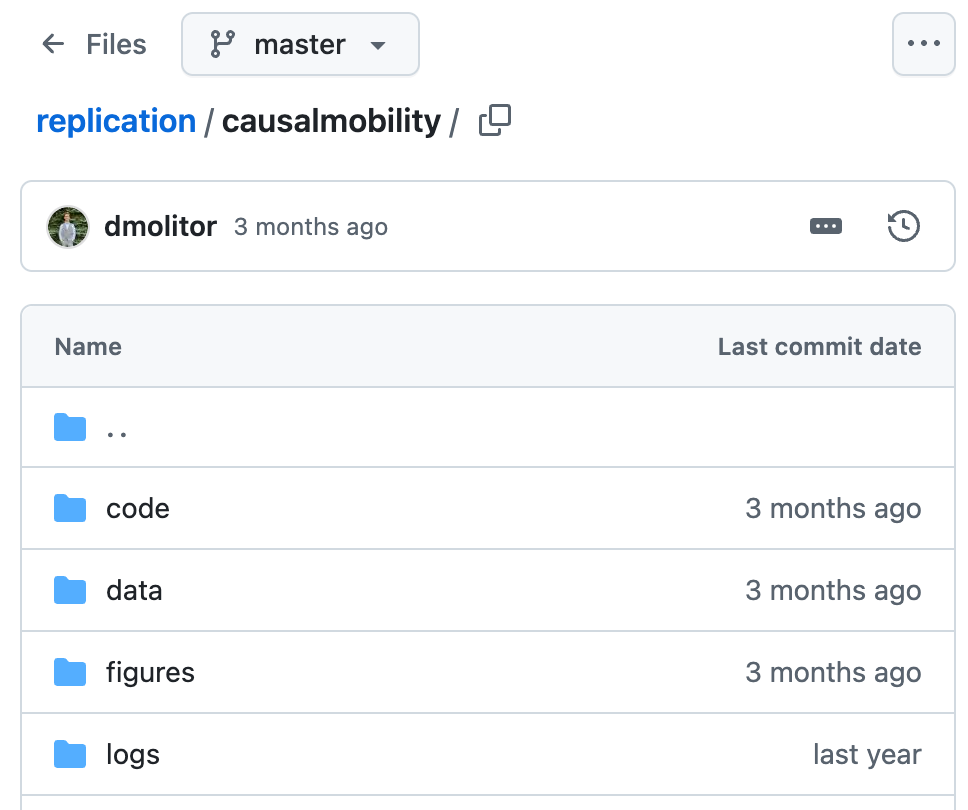
\includegraphics[height = .7\textheight]{figures/file_structure}}
\end{center}

\end{frame}

\begin{frame}{Organizing your workflow: Quarto documents}

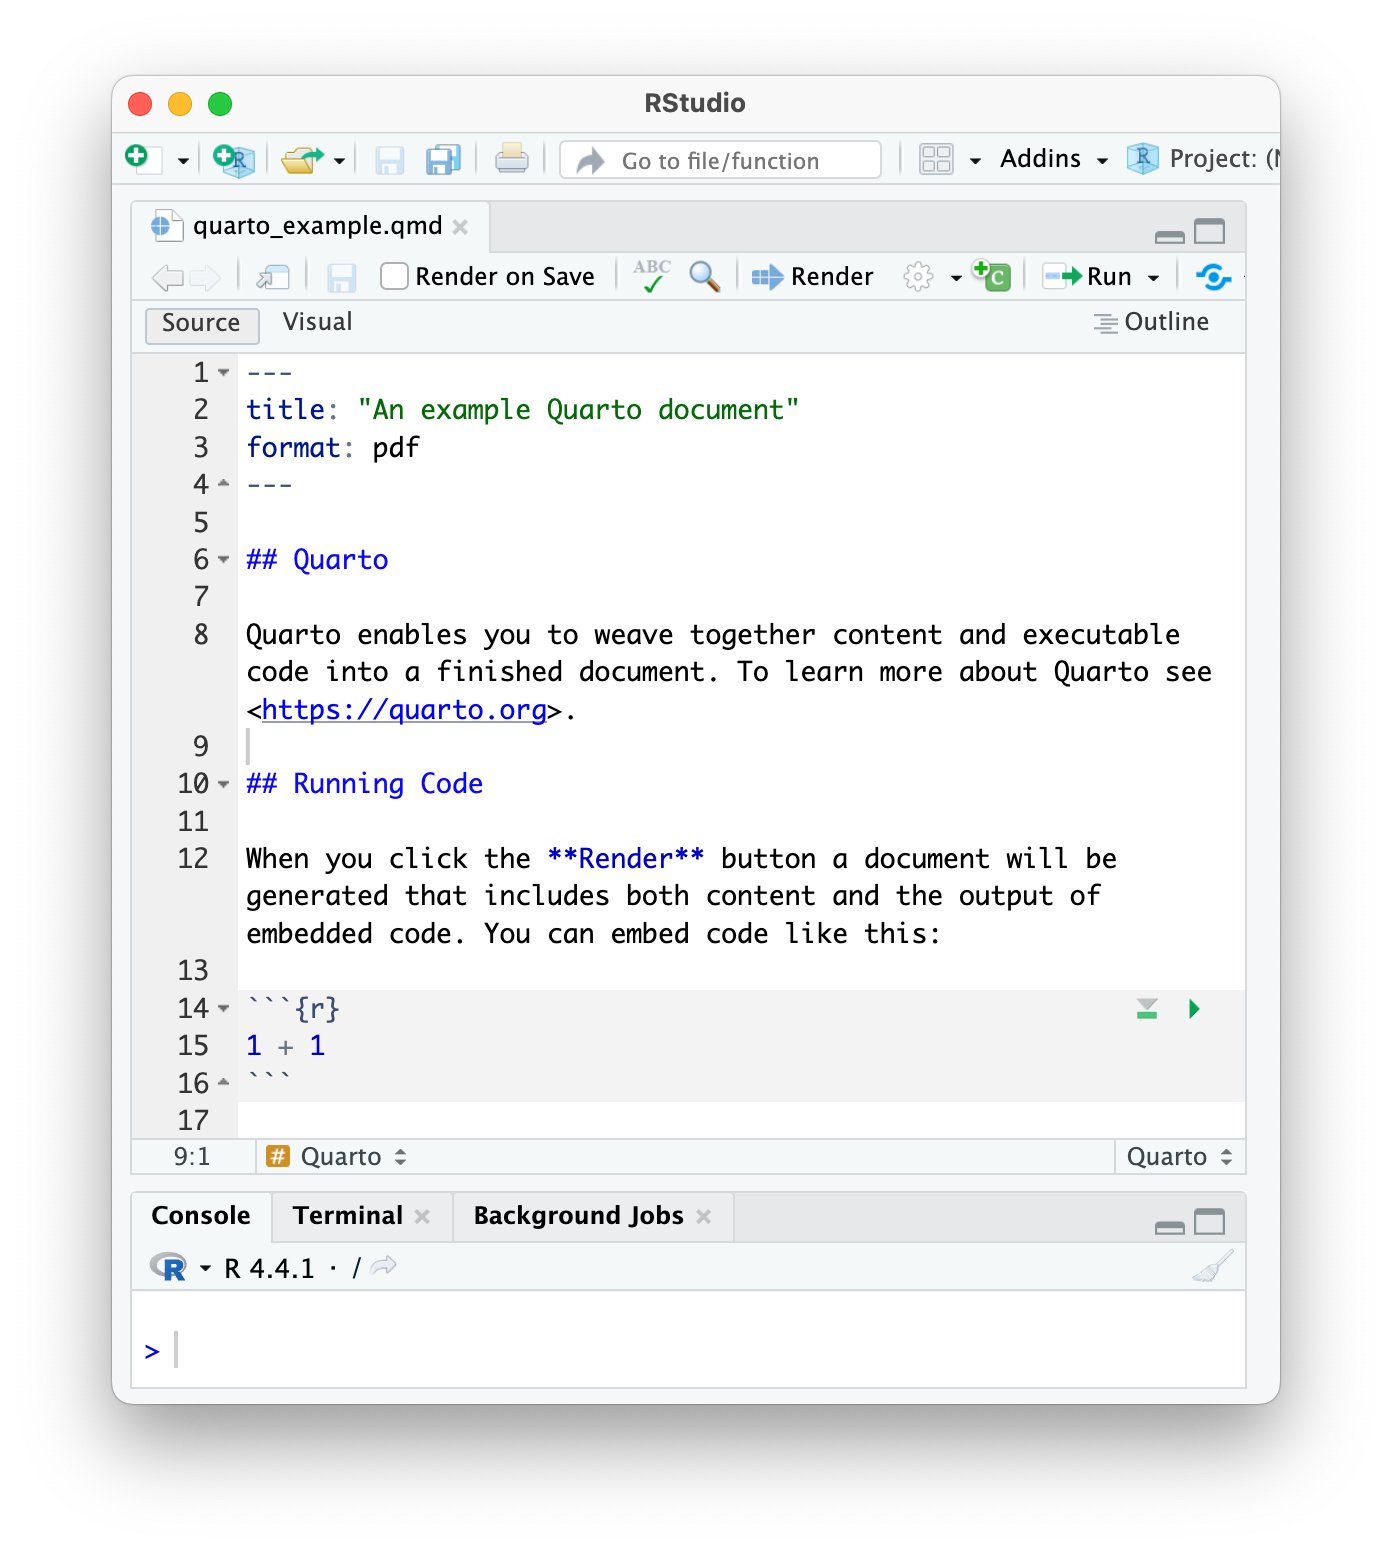
\includegraphics[width = .5\textwidth]{figures/quarto_code}
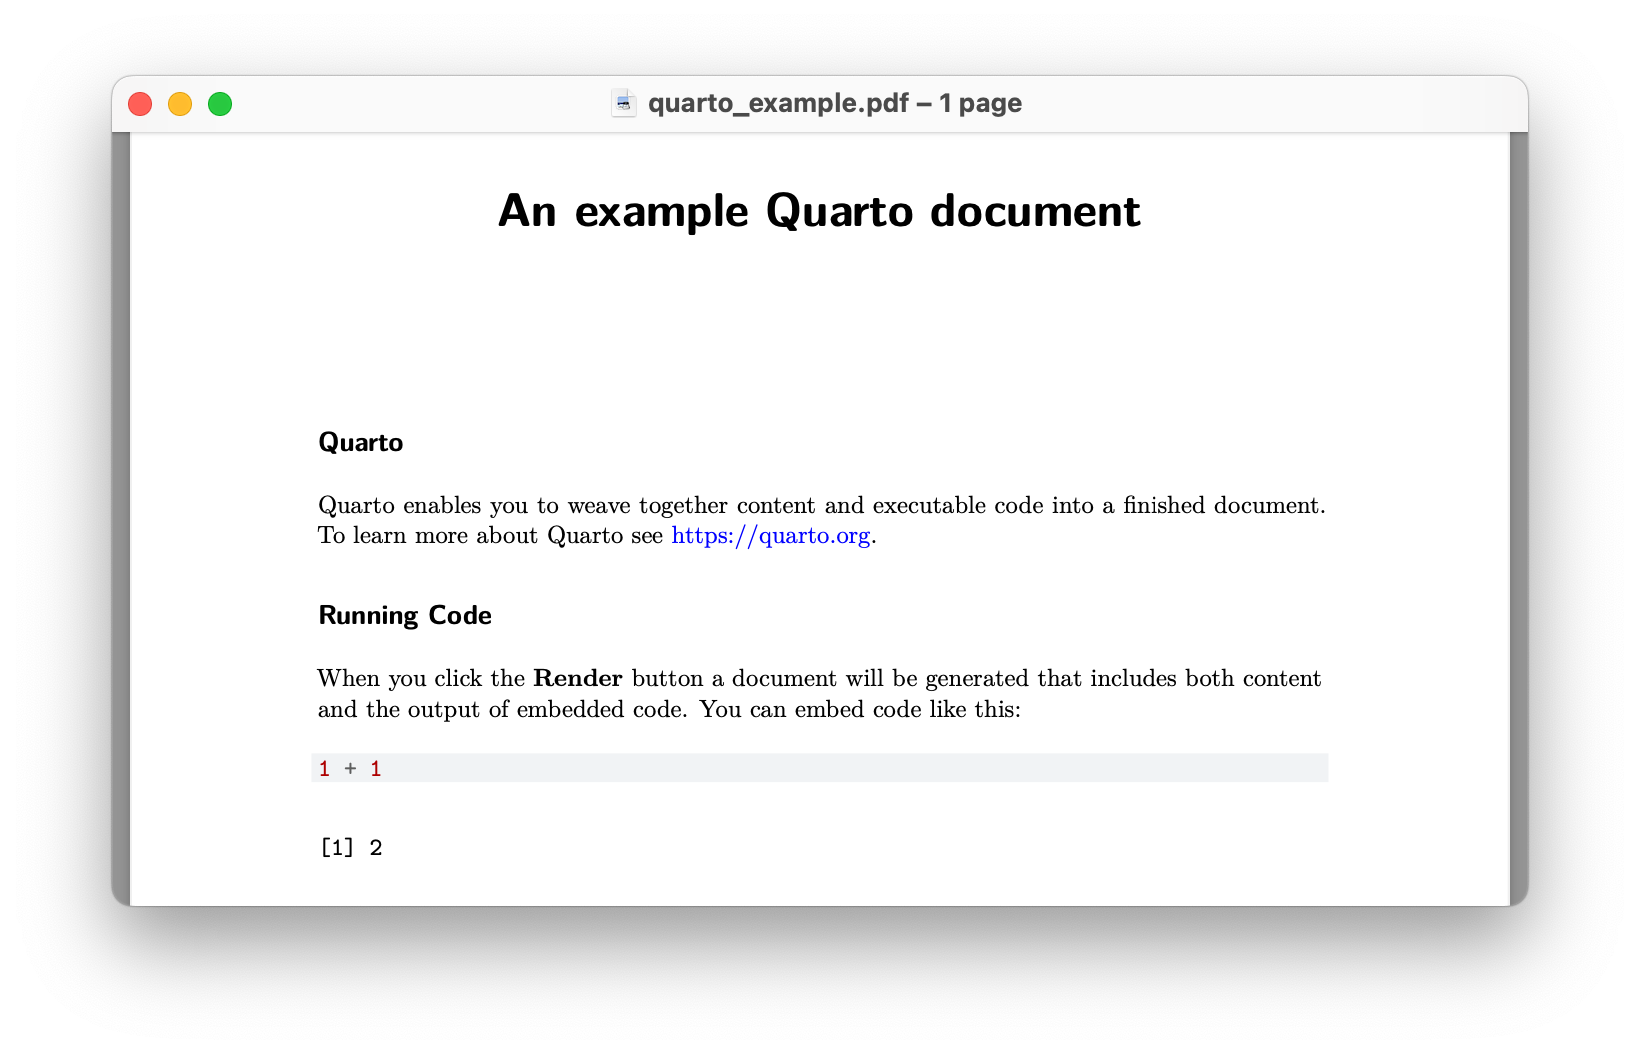
\includegraphics[width = .48\textwidth]{figures/quarto_document}

see the \bref{https://quarto.org/docs/get-started/hello/rstudio.html}{RStudio Quarto tutorial}

\end{frame}

\goalsframe

\end{document}